\chapter{Свидетельства о регистрации программы для ЭВМ}
\label{app:certificates}

\begin{center}
    
\includegraphics[height=0.8\textheight]{images/2024611544_program_registration.pdf}
\end{center}

\includepdf[pages=-]{images/2026618647_program_registration.pdf}

\chapter{Акт о внедрении}
\label{app:implementation}

\begin{center}
    
\includegraphics[height=0.8\textheight]{images/implementation}
\end{center}


\chapter{Интерфейс программы}\label{app:progrma_gui}

\begin{center}
    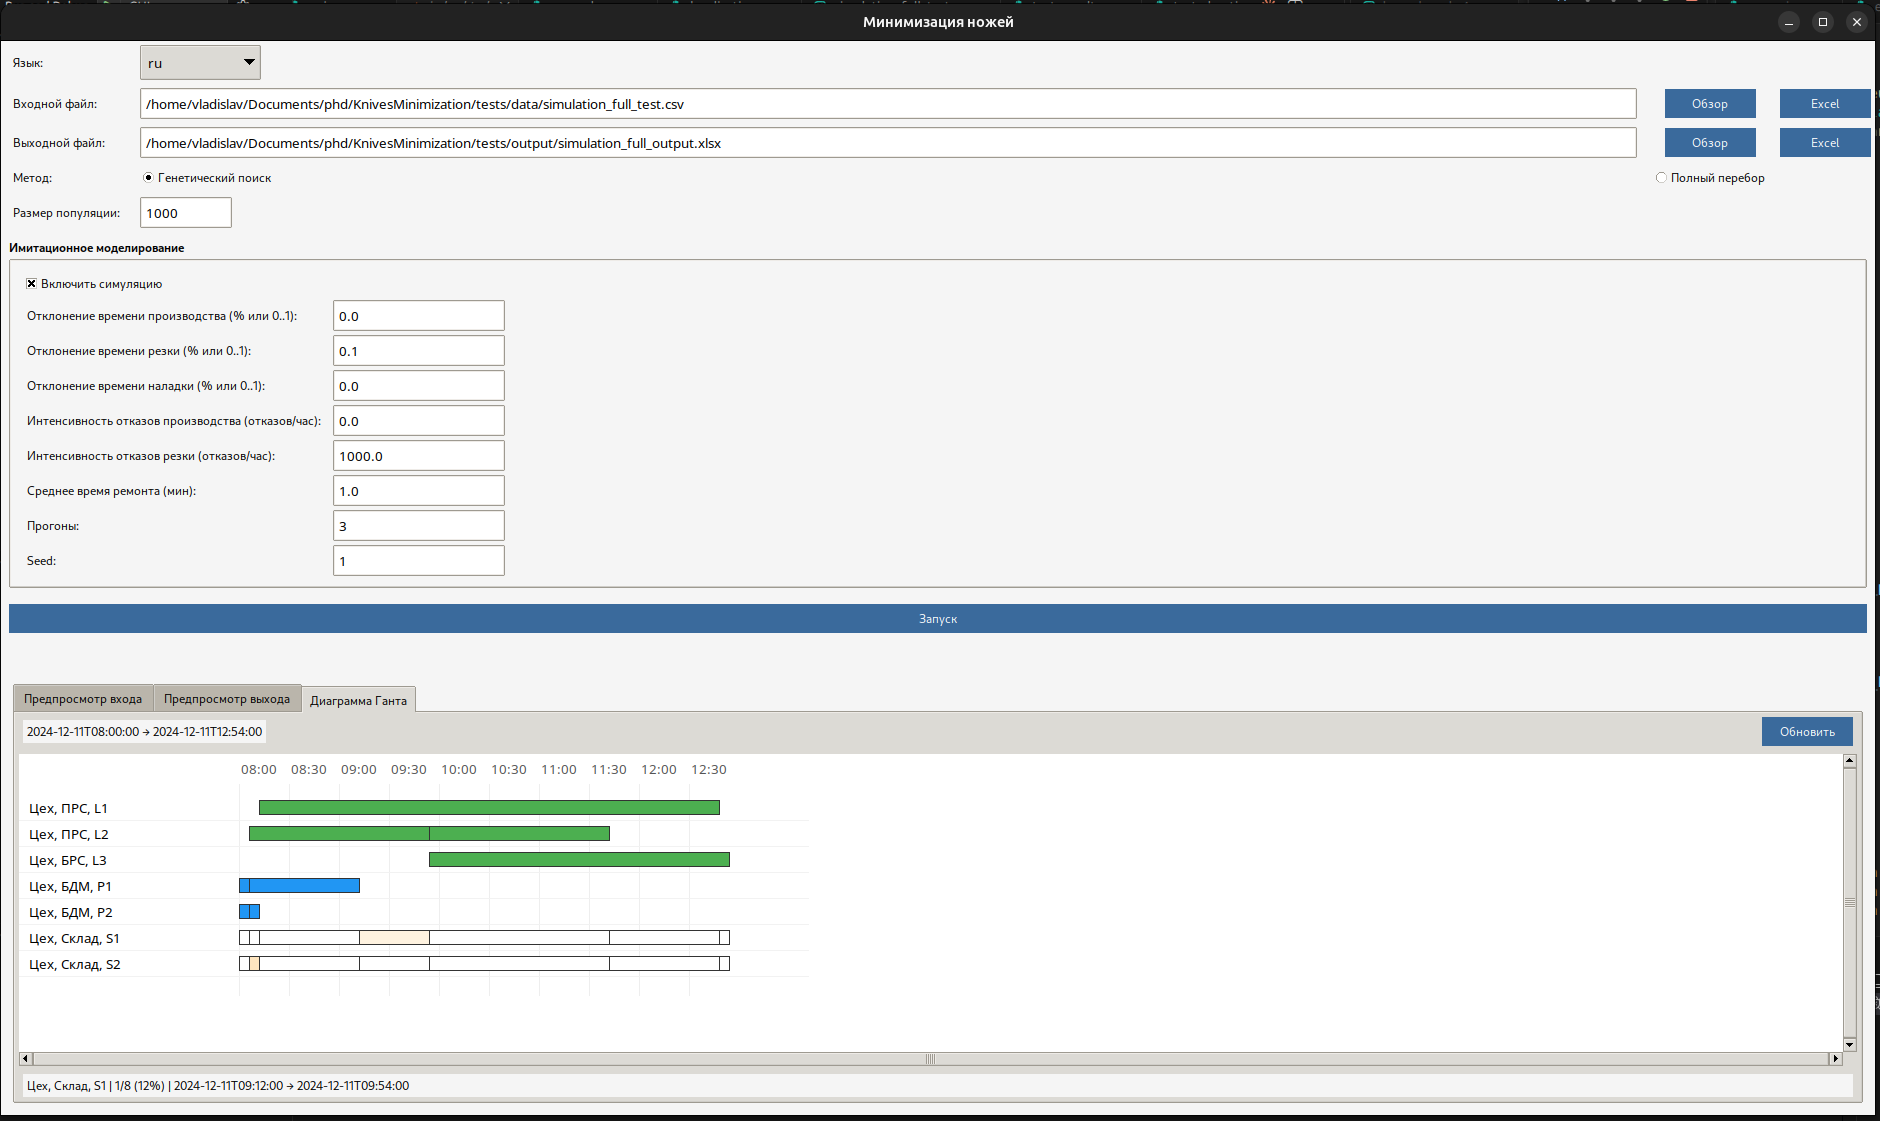
\includegraphics[width=\textwidth]{Dissertation/images/program/main.png}
    \captionof{figure}{Основной интерфейс программы}
    \label{fig:main_gui}
\end{center}

\begin{center}
    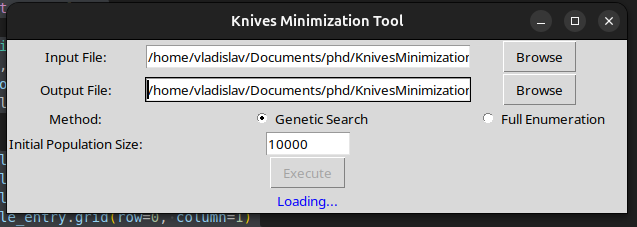
\includegraphics[width=\textwidth]{Dissertation/images/program/main_in_progress.png}
    \captionof{figure}{Интерфейс программы в процессе выполнения}
    \label{fig:main_in_progress}
\end{center}


\begin{center}
    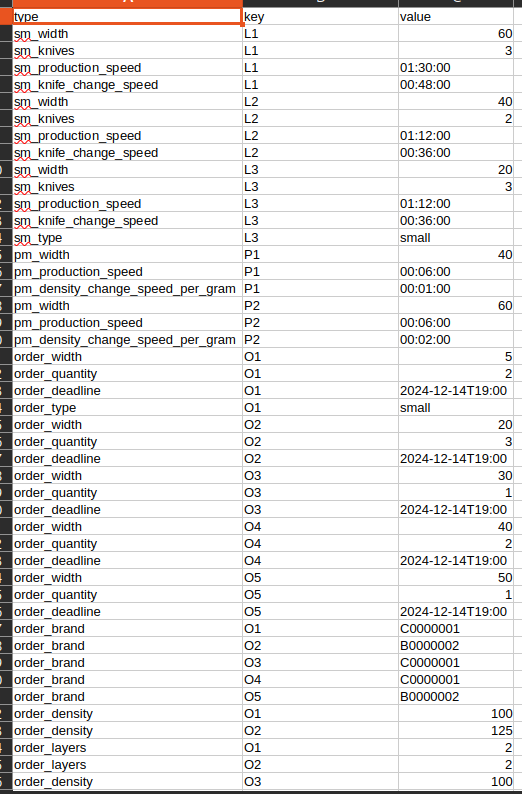
\includegraphics[height=0.95\textheight]{Dissertation/images/program/input_csv.png}
    \captionof{figure}{CSV-файл с вводными данными}
    \label{fig:input_csv}
\end{center}


\begin{center}
    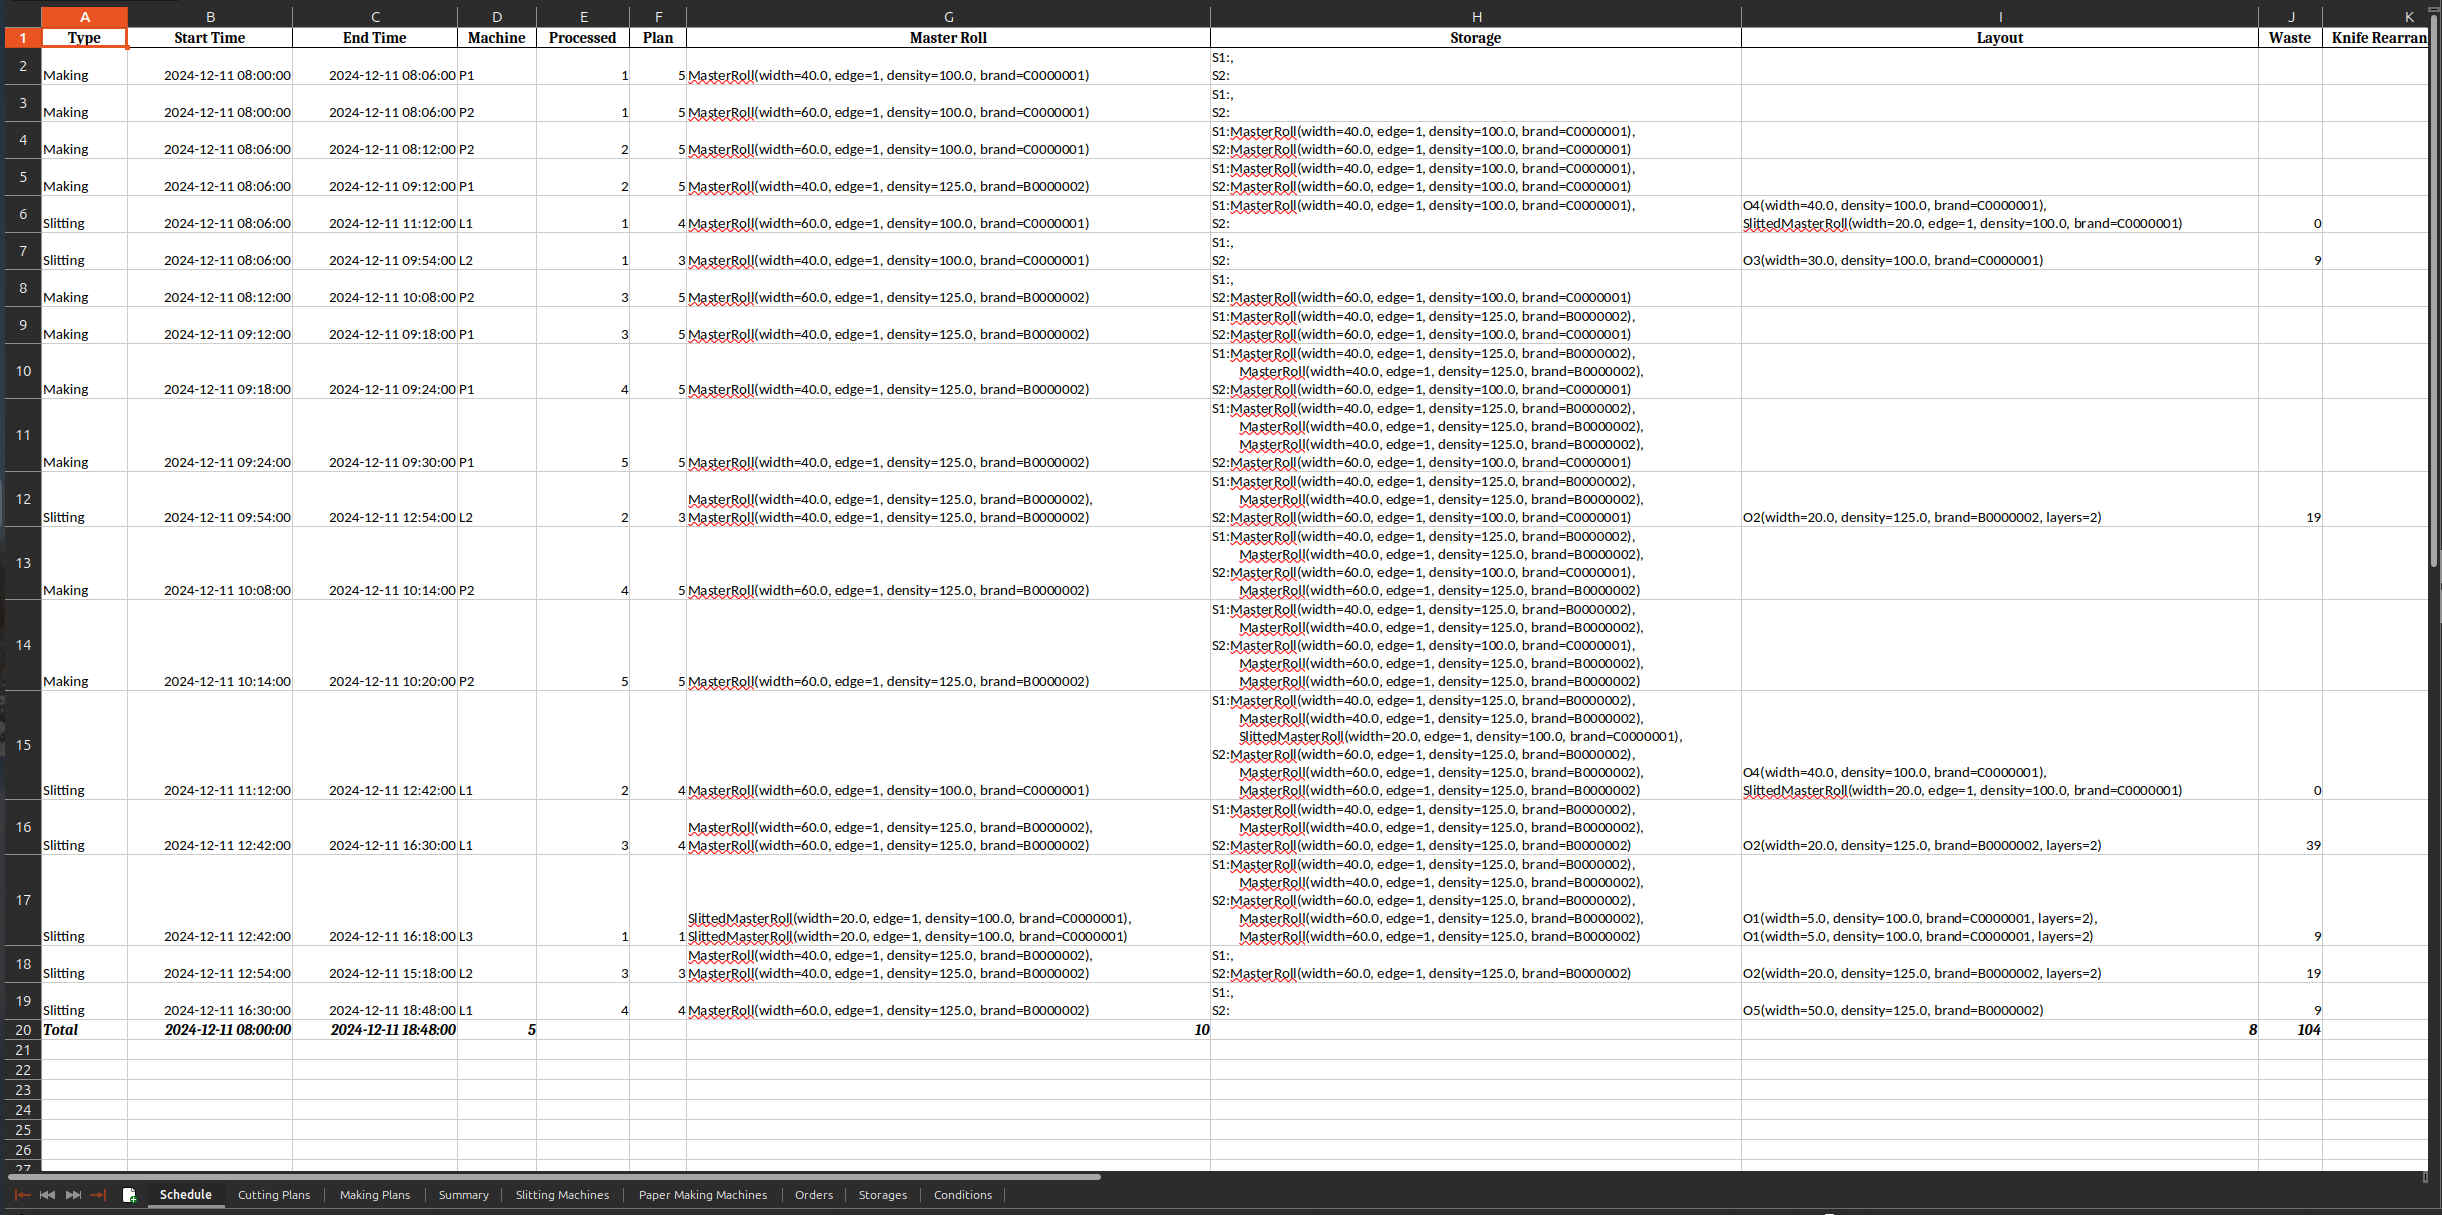
\includegraphics[width=\textwidth]{Dissertation/images/program/output_schedule.png}
    \captionof{figure}{Вкладка расписания выходного XLSX-файла}
    \label{fig:output_schedule}
\end{center}

\begin{center}
    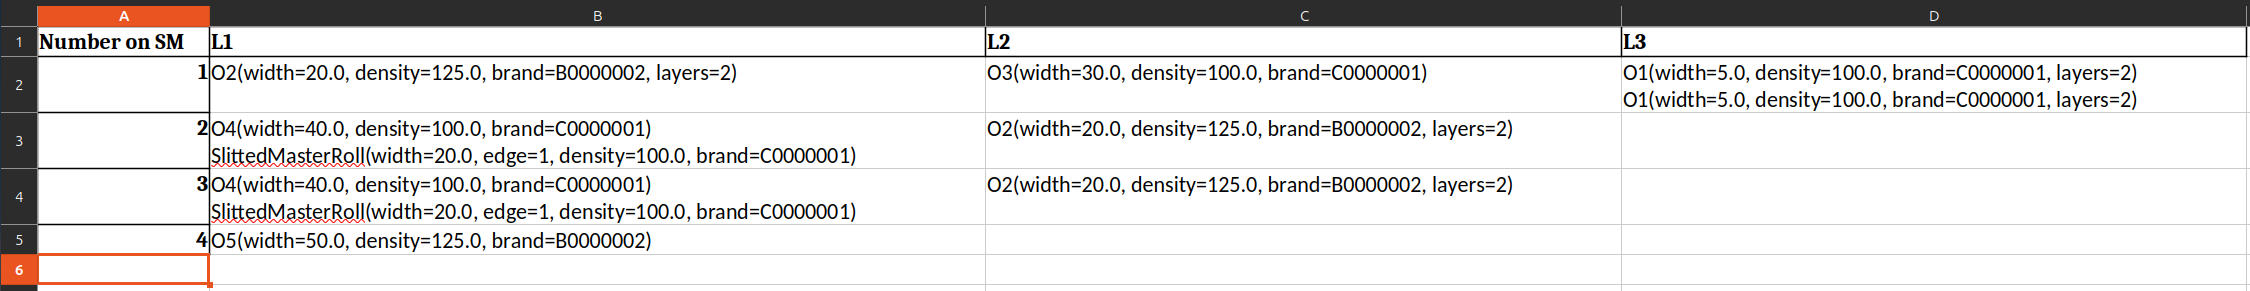
\includegraphics[width=\textwidth]{Dissertation/images/program/output_cutting_plans.png}
    \captionof{figure}{Вкладка планов нарезки выходного XLSX-файла}
    \label{fig:output_cutting_plans}
\end{center}
\begin{center}
    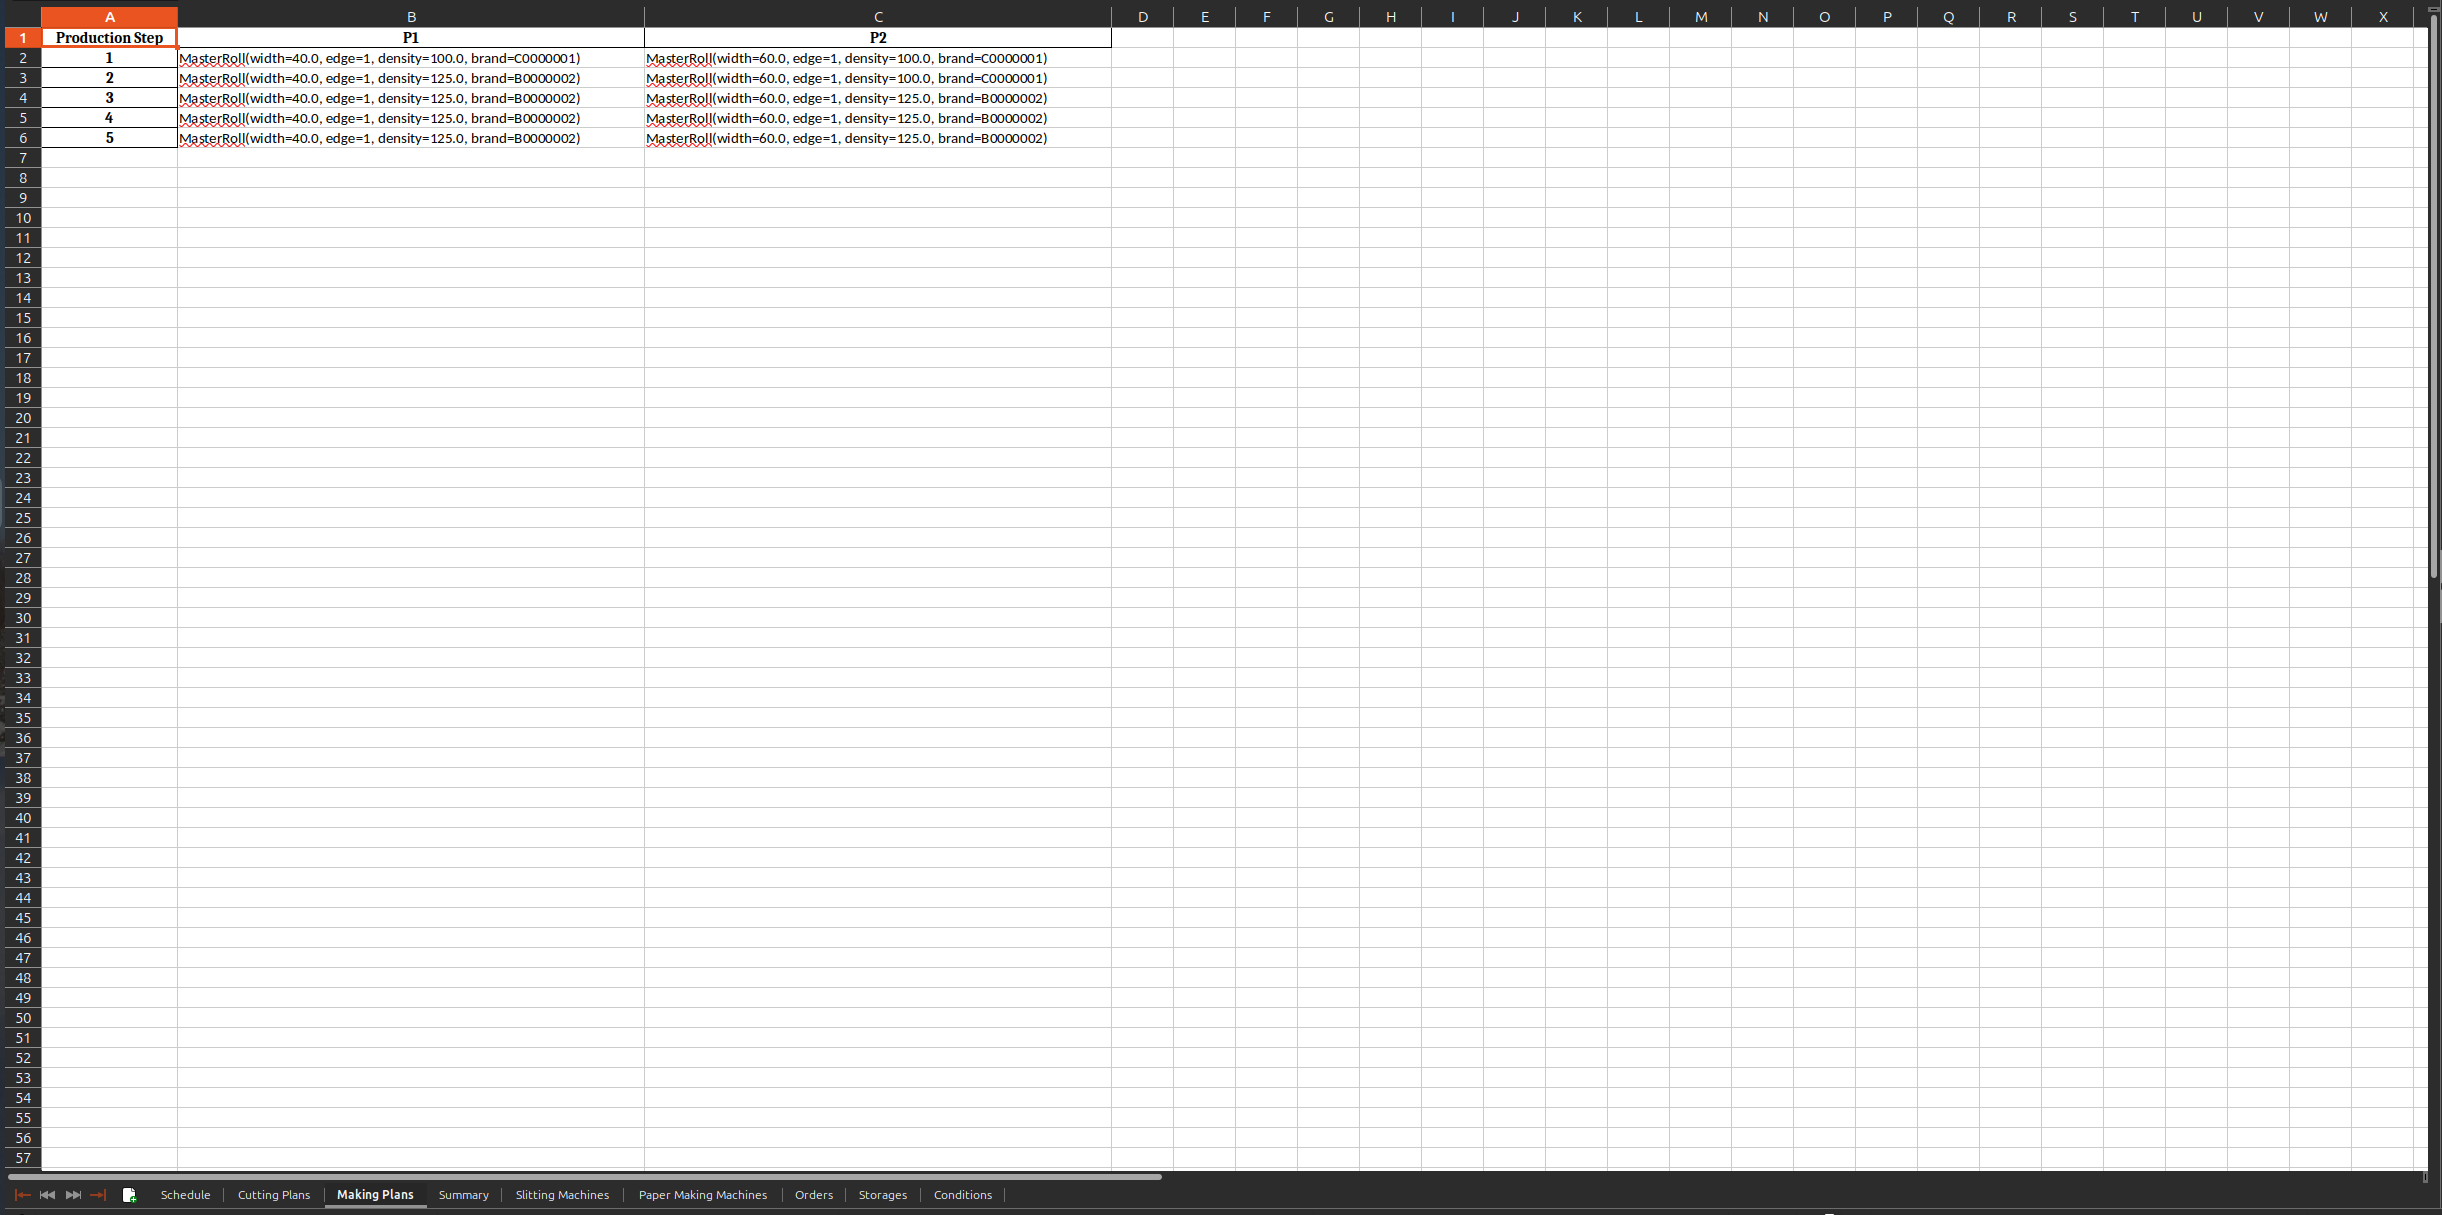
\includegraphics[width=\textwidth]{Dissertation/images/program/output_making_plans.png}
    \captionof{figure}{Вкладка планов производства выходного XLSX-файла}
    \label{fig:output_making_plans}
\end{center}
\begin{center}
    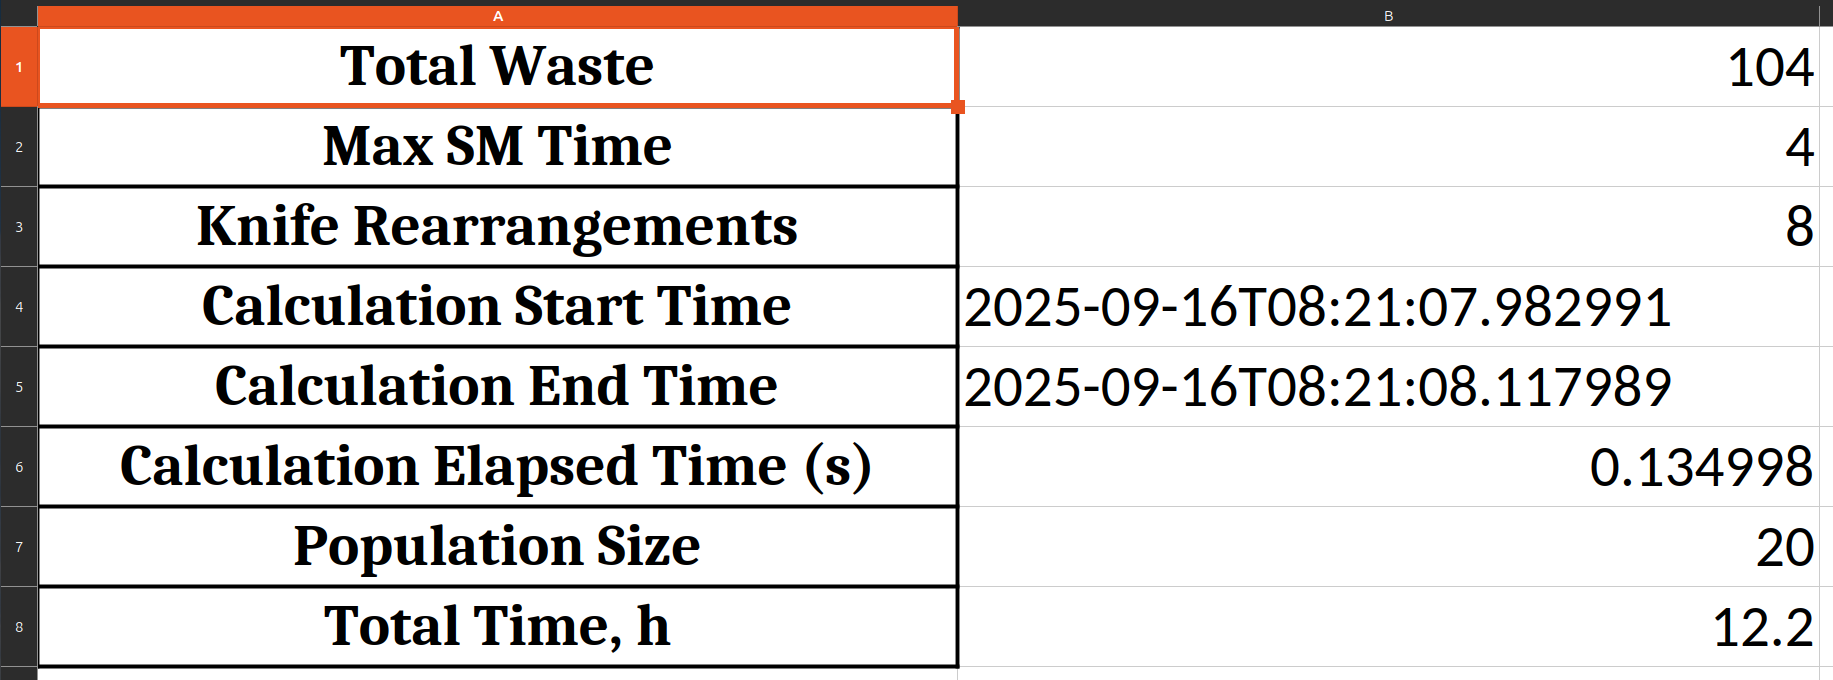
\includegraphics[width=\textwidth]{Dissertation/images/program/output_summary.png}
    \captionof{figure}{Вкладка с итогами выходного XLSX-файла}
    \label{fig:output_summary}
\end{center}

\begin{center}
    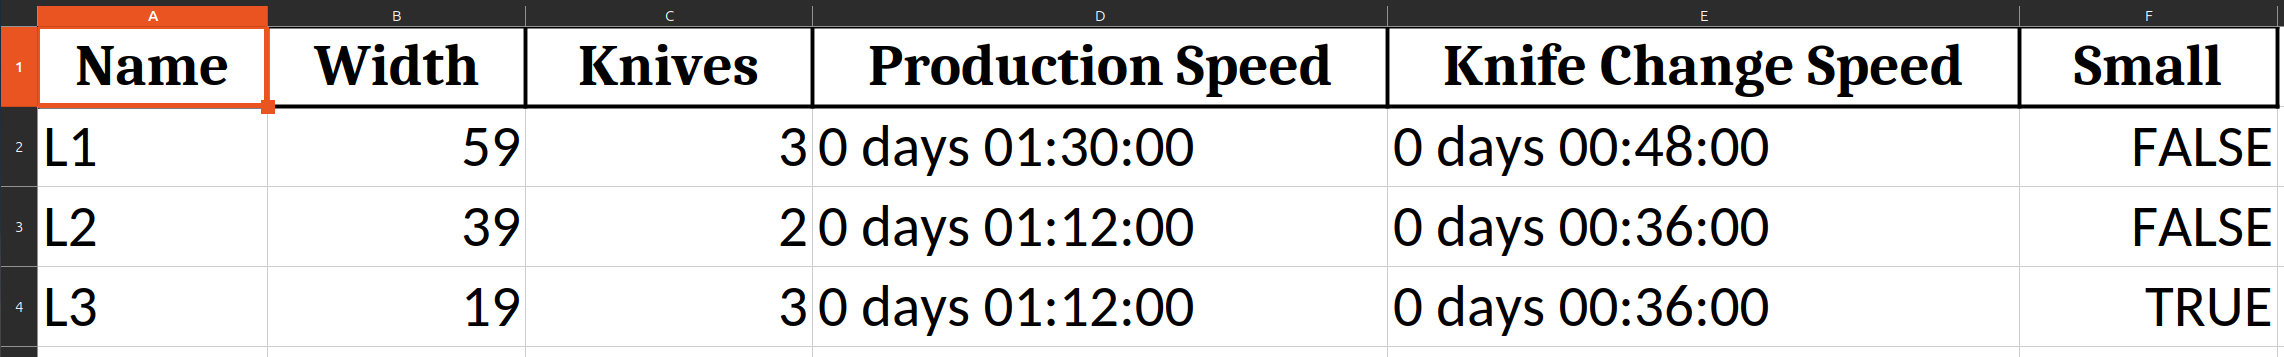
\includegraphics[width=\textwidth]{Dissertation/images/program/output_slitting_machines.png}
    \captionof{figure}{Вкладка с ПРС выходного XLSX-файла}
    \label{fig:output_slitting_machines}
\end{center}
\begin{center}
    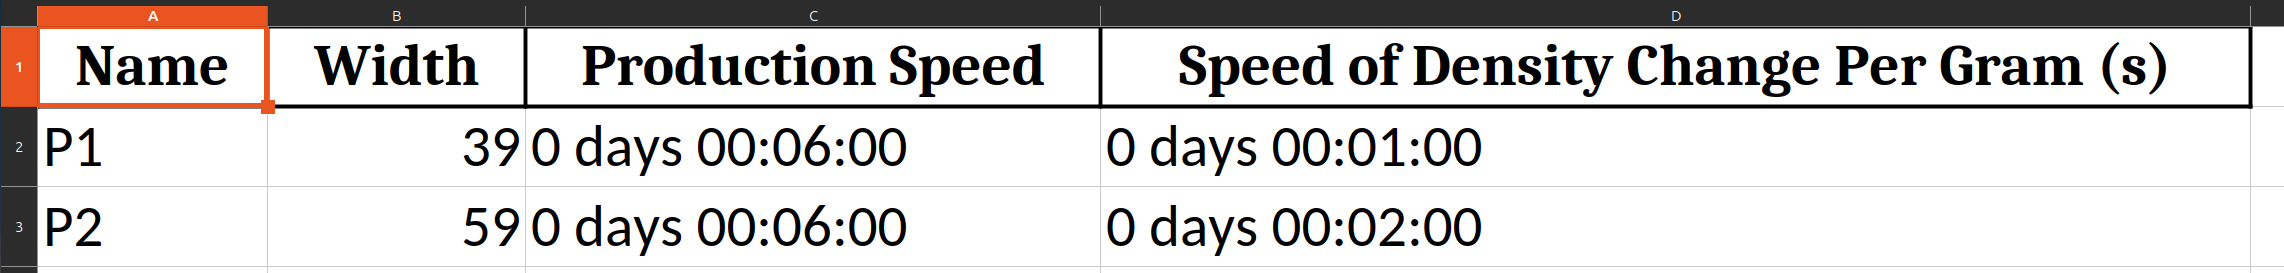
\includegraphics[width=\textwidth]{Dissertation/images/program/output_paper_making_machines.png}
    \captionof{figure}{Вкладка с БДМ выходного XLSX-файла}
    \label{fig:output_paper_making_machines}
\end{center}

\begin{center}
    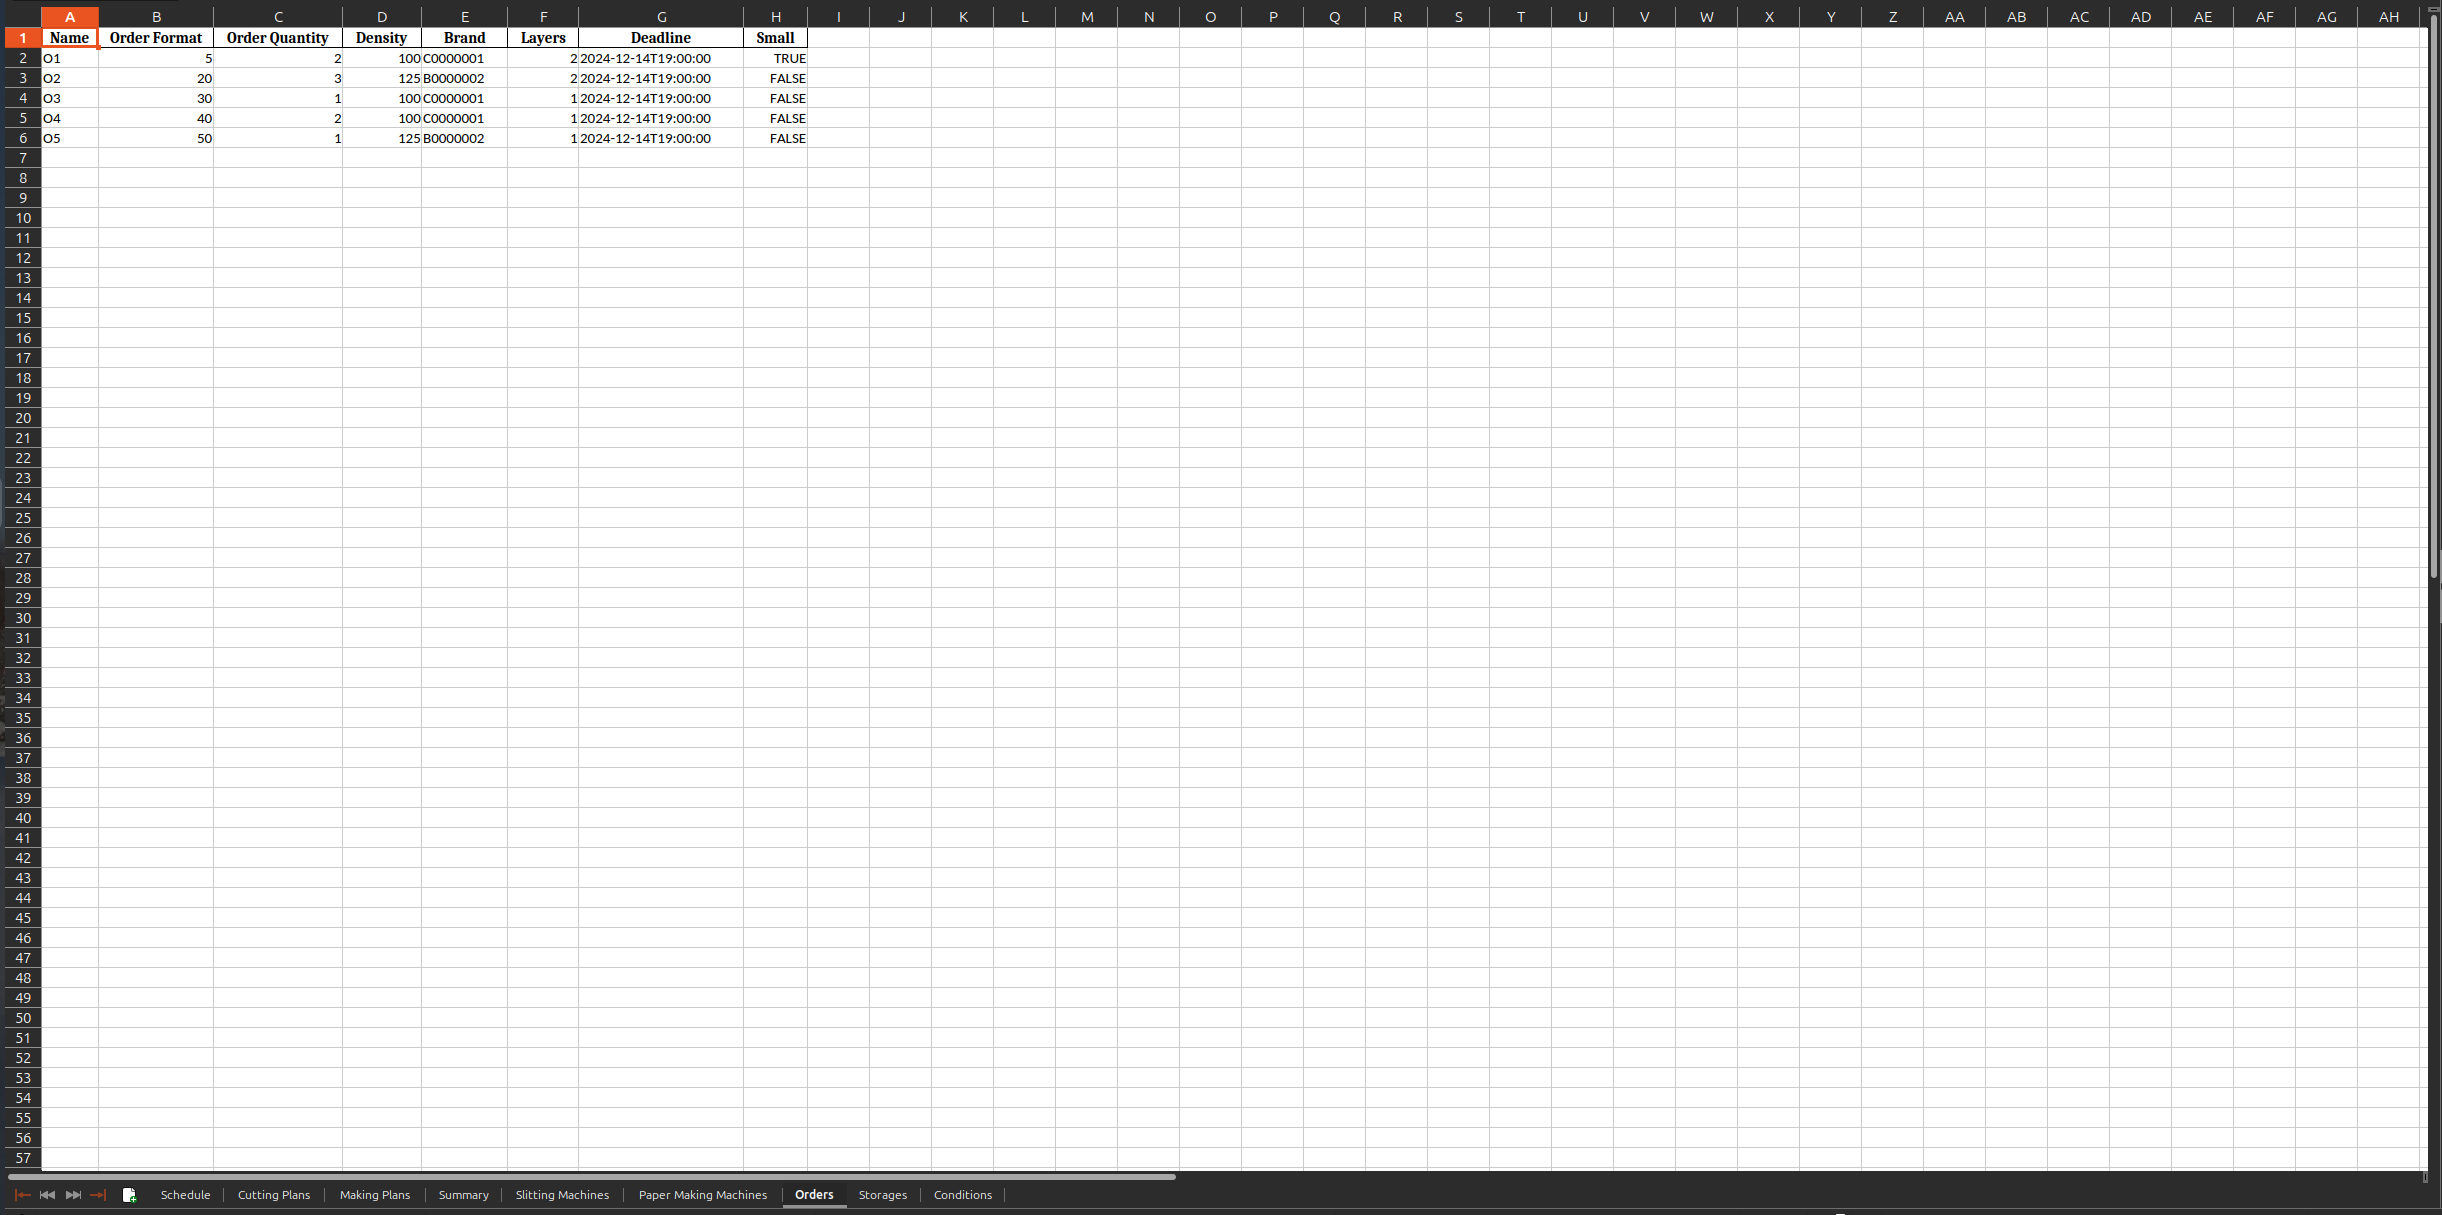
\includegraphics[width=\textwidth]{Dissertation/images/program/output_orders.png}
    \captionof{figure}{Вкладка заказы выходного XLSX-файла}
    \label{fig:output_orders}
\end{center}

\begin{center}
    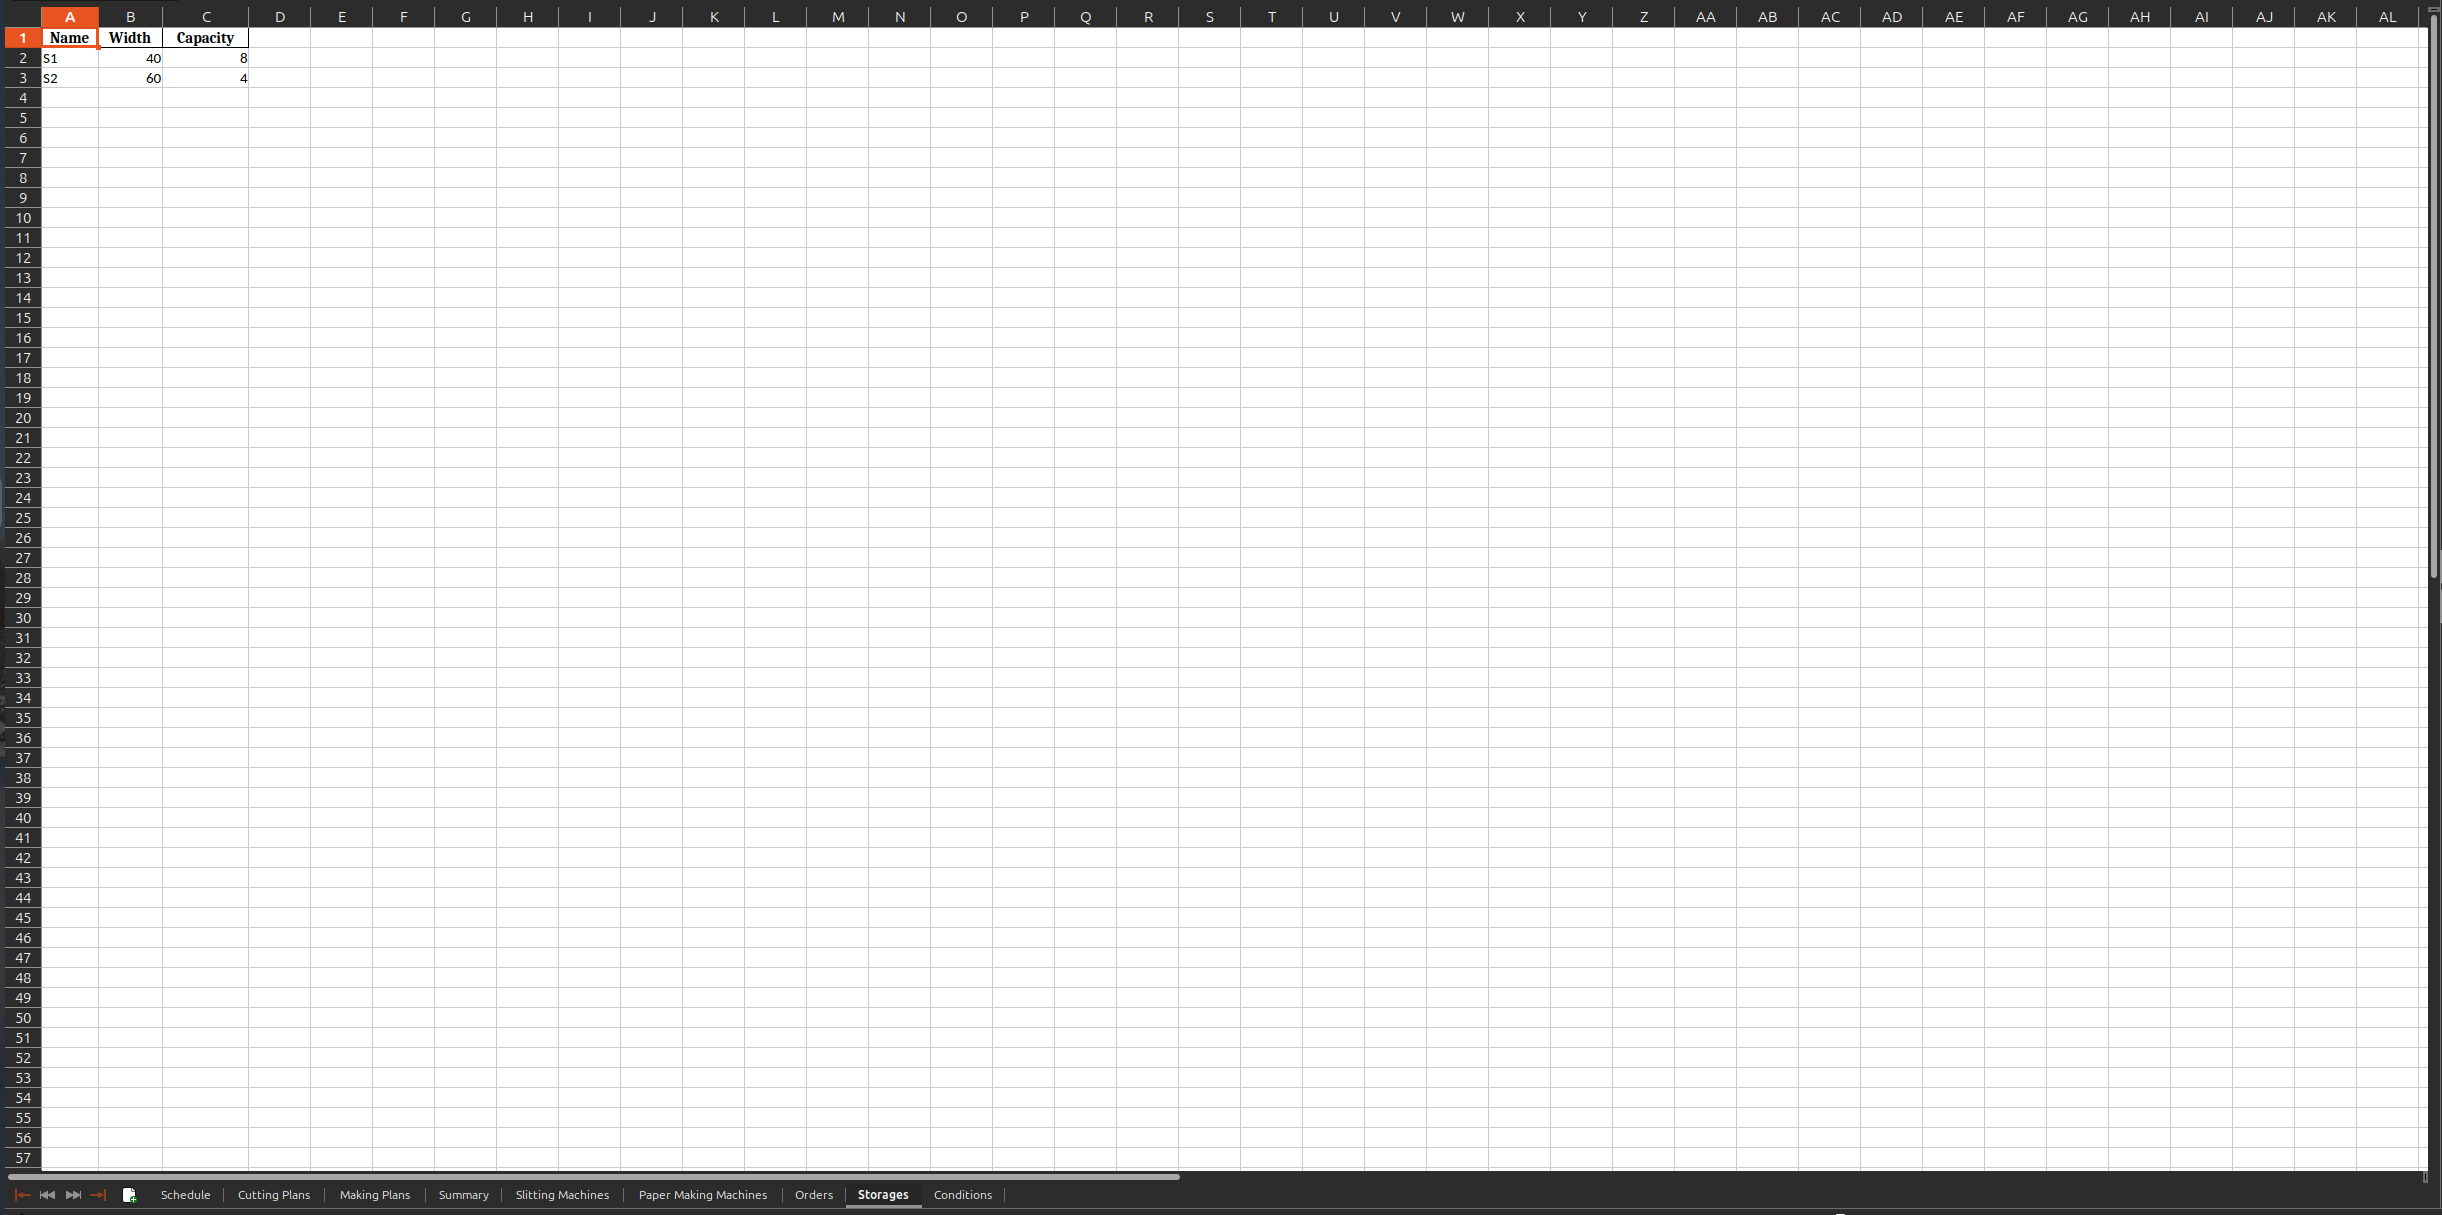
\includegraphics[width=\textwidth]{Dissertation/images/program/output_storages.png}
    \captionof{figure}{Вкладка со складами выходного XLSX-файла}
    \label{fig:output_storages}
\end{center}

\begin{center}
    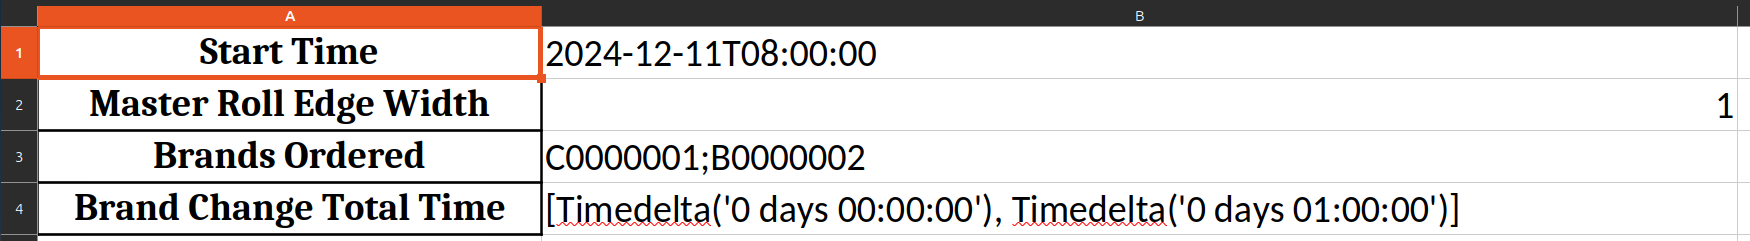
\includegraphics[width=\textwidth]{Dissertation/images/program/output_conditions.png}
    \captionof{figure}{Вкладка с общими улсловиями задачи выходного XLSX-файла}
    \label{fig:output_conditions}
\end{center}

\chapter{Спецификация тестов}
\label{app:testing-specification}

\section{Тесты модельного слоя (\texttt{models/tests})}
\paragraph{test\_cutting\_layout.py}
\begin{itemize}
    \item \textbf{test\_cutting\_layout} --- проверяет валидность раскроя при
    разных ширинах и числе ножей, а также вычисление отходов.
    \item \textbf{test\_format\_dicts} --- проверяет корректность словаря форматов
    (количество рулонов одного типа в раскрое).
\end{itemize}

\paragraph{test\_cutting\_plan.py}
\begin{itemize}
    \item \textbf{test\_cutting\_plan} --- проверяет валидность плана и расчет
    отходов и перестановок ножей.
    \item \textbf{test\_formats\_dict} --- проверяет распределение заказов по плану.
    \item \textbf{test\_total\_speed\_cutting\_plan} --- проверяет расчет времени
    раскроя с учетом скорости производства и перестановок.
    \item \textbf{test\_total\_speed\_layered\_cutting\_plan} --- проверяет
    корректность времени при многослойных заказах.
\end{itemize}

\paragraph{test\_global\_plan.py}
\begin{itemize}
    \item \textbf{test\_formats\_dict} --- проверяет корректность агрегирования
    количества заказов по всему глобальному плану.
    \item \textbf{test\_good\_global\_plan} --- проверяет корректность базового
    глобального плана, его отходов и перестановок.
    \item \textbf{test\_article\_global\_plan} --- проверяет пример плана из
    статьи (ожидаемые метрики).
    \item \textbf{test\_article\_solution\_global\_plan} --- проверяет
    эталонное решение из статьи.
    \item \textbf{test\_article\_best\_global\_plan} --- проверяет план с
    нулевыми отходами и минимальными перестановками.
    \item \textbf{test\_global\_plan\_comparison} --- проверяет корректность
    сравнения планов по критериям.
    \item \textbf{test\_max\_slitting\_machine\_plans} --- проверяет расчет
    максимального числа раскроев на станке.
\end{itemize}

\paragraph{test\_making\_plan.py}
\begin{itemize}
    \item \textbf{test\_making\_plan\_total\_time} --- проверяет расчет времени
    производства тамбуров.
    \item \textbf{test\_making\_plan\_equality} --- проверяет сравнение планов
    по количеству тамбуров.
    \item \textbf{test\_making\_plan\_string\_representation} --- проверяет
    строковое представление плана.
\end{itemize}

\paragraph{test\_problem.py}
\begin{itemize}
    \item \textbf{test\_one\_plus\_one} --- проверка корректности тестовой
    инфраструктуры.
    \item \textbf{test\_problem} --- проверяет базовую корректность объекта
    задачи (число заказов и станков).
    \item \textbf{test\_problem\_with\_knives\_and\_speed} --- проверяет загрузку
    параметров станков (ножи и скорости).
\end{itemize}

\paragraph{test\_roll.py}
\begin{itemize}
    \item \textbf{test\_is\_compatible} --- проверяет совместимость рулонов по
    количеству слоев.
\end{itemize}



\section{Тесты алгоритмического модуля (\texttt{algo/tests})}

\paragraph{test\_crossingover.py}
\begin{itemize}
    \item \textbf{test\_crossingover} --- проверяет, что оператор кроссинговера
    возвращает один из двух входных глобальных планов и не ухудшает их метрики
    (отходы и перестановки ножей).
\end{itemize}

\paragraph{test\_event\_queue\_builder.py}
\begin{itemize}
    \item \textbf{test\_total\_speed\_global\_plan} --- проверяет, что общее время
    выполнения глобального плана совпадает с максимальным временем раскроя на
    отдельных станках.
    \item \textbf{test\_global\_plan\_time\_limit} --- проверяет корректность
    обработки дедлайнов: при слишком жестких сроках план становится недопустимым.
    \item \textbf{test\_pms\_global\_plan\_time\_limit} --- аналогичная проверка,
    но с учетом бумагоделательных машин и сформированных производственных планов.
    \item \textbf{test\_global\_plan\_with\_storage\_capacity} --- проверяет, что
    расписание учитывает ограничения склада и включает моменты ожидания, если
    нет доступных рулонов.
\end{itemize}

\paragraph{test\_full\_enumeration.py}
\begin{itemize}
    \item \textbf{test\_full\_enumeration} --- проверяет, что полный перебор
    возвращает корректное решение, не хуже случайных планов.
    \item \textbf{test\_article\_best\_solution} --- проверяет соответствие
    результату для примера из статьи: найденное решение не хуже эталонного.
\end{itemize}

\paragraph{test\_genetic\_search.py}
\begin{itemize}
    \item \textbf{test\_genetic\_search} --- проверяет, что генетический поиск
    возвращает корректный план и улучшает качество по сравнению со случайными
    решениями.
\end{itemize}

\paragraph{test\_global\_mutate.py}
\begin{itemize}
    \item \textbf{test\_global\_mutate} --- проверяет, что глобальная мутация
    не ухудшает решение и иногда улучшает его.
    \item \textbf{test\_event\_rebuild} --- проверяет, что после мутации очередь
    событий пересчитывается (операции могут отличаться по времени или типу).
\end{itemize}

\paragraph{test\_mutate.py}
\begin{itemize}
    \item \textbf{test\_mutate} --- проверяет, что локальная мутация плана
    раскроя действительно меняет конфигурацию (перестановка форматов/раскроев).
\end{itemize}

\paragraph{test\_pmm\_plans\_builder.py}
\begin{itemize}
    \item \textbf{test\_generate\_making\_plans\_simple\_case} --- проверяет
    корректное формирование плана производства тамбуров для одной БДМ.
    \item \textbf{test\_generate\_making\_plans\_multiple\_identical\_machines} ---
    проверяет распределение тамбуров между несколькими одинаковыми БДМ.
    \item \textbf{test\_generate\_making\_plans\_different\_widths} --- проверяет
    соответствие ширин тамбуров и БДМ при нескольких типах машин.
    \item \textbf{test\_total\_time\_pms\_global\_plan} --- проверяет корректность
    вычисления суммарного времени плана при наличии БДМ.
\end{itemize}

\paragraph{test\_random\_global\_plan.py}
\begin{itemize}
    \item \textbf{test\_randomness} --- проверяет, что генератор случайных планов
    формирует различающиеся решения.
    \item \textbf{test\_constraints} --- проверяет выполнение ограничений в
    случайных планах.
    \item \textbf{test\_constraints\_strictly} --- аналогичная проверка при
    строгой конфигурации ширин станков.
    \item \textbf{test\_invalid} --- проверяет, что при невозможности решения
    генерация плана вызывает исключение.
    \item \textbf{test\_time\_pms} --- проверяет корректность планов при наличии
    БДМ и временных ограничений.
    \item \textbf{test\_density} --- проверяет, что в раскрое сохраняется
    однородность плотности рулонов.
\end{itemize}

\section{Тесты ввода/вывода (\texttt{inoutput/tests})}

\paragraph{test\_input.py}
\begin{itemize}
    \item \textbf{test\_parse\_input} --- проверяет базовый парсинг CSV.
    \item \textbf{test\_parse\_input\_with\_knives} --- проверяет парсинг ножей.
    \item \textbf{test\_parse\_input\_with\_additional\_attributes} --- проверяет
    чтение скоростей производства и перестановки ножей.
    \item \textbf{test\_parse\_input\_with\_time\_limit} --- проверяет чтение
    дедлайнов и времени запуска.
    \item \textbf{test\_parse\_input\_with\_paper\_making\_machines} --- проверяет
    парсинг БДМ и их параметров.
    \item \textbf{test\_storage\_capacity\_input} --- проверяет парсинг складов.
    \item \textbf{test\_parse\_orders\_with\_density} --- проверяет чтение плотности.
    \item \textbf{test\_parse\_orders\_with\_density\_change\_speed} --- проверяет
    чтение скорости смены плотности на БДМ.
    \item \textbf{test\_parse\_brand} --- проверяет чтение марки бумаги.
    \item \textbf{test\_parse\_brand\_ordered} --- проверяет чтение порядка марок
    и времени переналадки.
    \item \textbf{test\_excel\_input} --- проверяет чтение Excel со всеми
    параметрами (станки, заказы, склад, марки).
    \item \textbf{test\_excel\_simple\_input} --- проверяет упрощенный Excel.
    \item \textbf{test\_layers\_input} --- проверяет чтение числа слоев.
    \item \textbf{test\_edge\_input} --- проверяет чтение кромки.
    \item \textbf{test\_small\_order\_input} --- проверяет чтение типа заказа
    (ПРС/БРС).
\end{itemize}

\paragraph{test\_output.py}
\begin{itemize}
    \item \textbf{test\_output\_solution} --- проверяет корректность CSV-вывода
    (сравнение с эталонным файлом).
    \item \textbf{test\_output\_solution\_excel} --- проверяет генерацию Excel
    отчета и его наличие.
\end{itemize}

\section{Интеграционные тесты (\texttt{tests/})}

\paragraph{test\_functional.py}
\begin{itemize}
    \item \textbf{test\_pmm} --- запуск полного цикла расчета с БДМ.
    \item \textbf{test\_pmm\_with\_time} --- запуск полного цикла с учетом времени.
    \item \textbf{test\_storage} --- проверка корректного ожидания при складских
    ограничениях.
    \item \textbf{test\_density} --- проверка согласованности плотности в планах.
    \item \textbf{test\_density\_with\_time} --- запуск задачи с плотностью и
    дедлайнами.
    \item \textbf{test\_brand} --- проверка согласованности марок.
    \item \textbf{test\_brand\_ordered} --- проверка соблюдения порядка марок.
    \item \textbf{test\_density\_brand} --- проверка совмещения плотности и марок.
    \item \textbf{test\_layers} --- запуск задачи со слоями.
    \item \textbf{test\_layers\_with\_time} --- слои с временными ограничениями.
    \item \textbf{test\_subslitting} --- проверка сценария БРС.
    \item \textbf{test\_subslitting\_with\_time} --- БРС с дедлайнами.
    \item \textbf{test\_edge} --- проверка корректной обработки кромки.
    \item \textbf{test\_full\_problem} --- полный интеграционный сценарий
    со всеми ограничениями.
\end{itemize}

\paragraph{test\_benchmark.py}
\begin{itemize}
    \item \textbf{test\_benchmark\_1\_full\_enumeration} --- бенчмарк с полным
    перебором (отключен по умолчанию).
    \item \textbf{test\_benchmark\_1\_genetic\_search} --- бенчмарк генетического
    поиска (отключен по умолчанию).
    \item \textbf{test\_benchmark\_2\_full\_enumeration} --- второй сценарий
    бенчмарка (отключен).
    \item \textbf{test\_benchmark\_2\_genetic\_search} --- второй сценарий для GA
    (отключен).
    \item \textbf{test\_benchmark\_3\_full\_enumeration} --- третий сценарий
    бенчмарка (отключен).
    \item \textbf{test\_benchmark\_3\_genetic\_search} --- третий сценарий для GA
    (отключен).
    \item \textbf{test\_benchmark\_4\_full\_enumeration} --- четвертый сценарий
    бенчмарка (отключен).
    \item \textbf{test\_benchmark\_4\_genetic\_search} --- четвертый сценарий для
    GA (отключен).
\end{itemize}
 
 
 \chapter{UML-схемы программного комплекса}
 \label{app:uml-diagrams}
 
 \begin{center}
     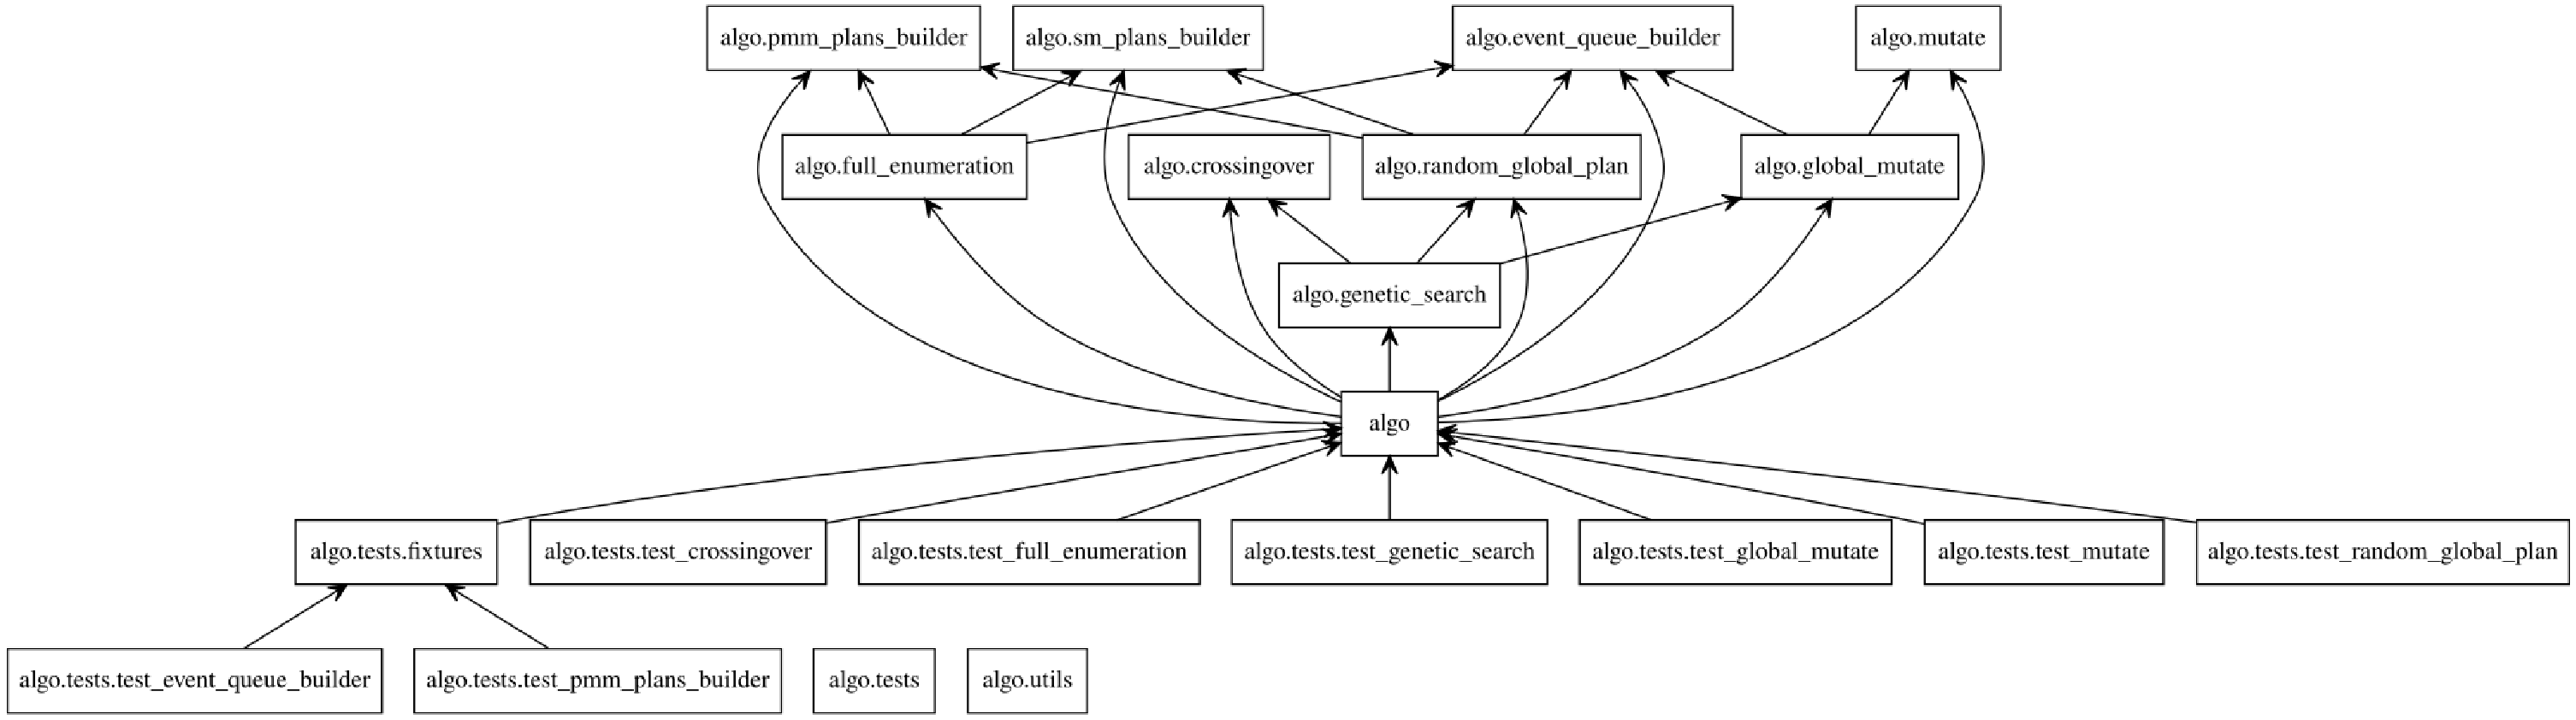
\includegraphics[width=\textwidth]{Dissertation/images/packages_algo.pdf}
     \captionof{figure}{UML-схема пакетов алгоритмического модуля \texttt{algo}}
     \label{fig:uml-packages-algo}
 \end{center}
 
 \begin{center}
     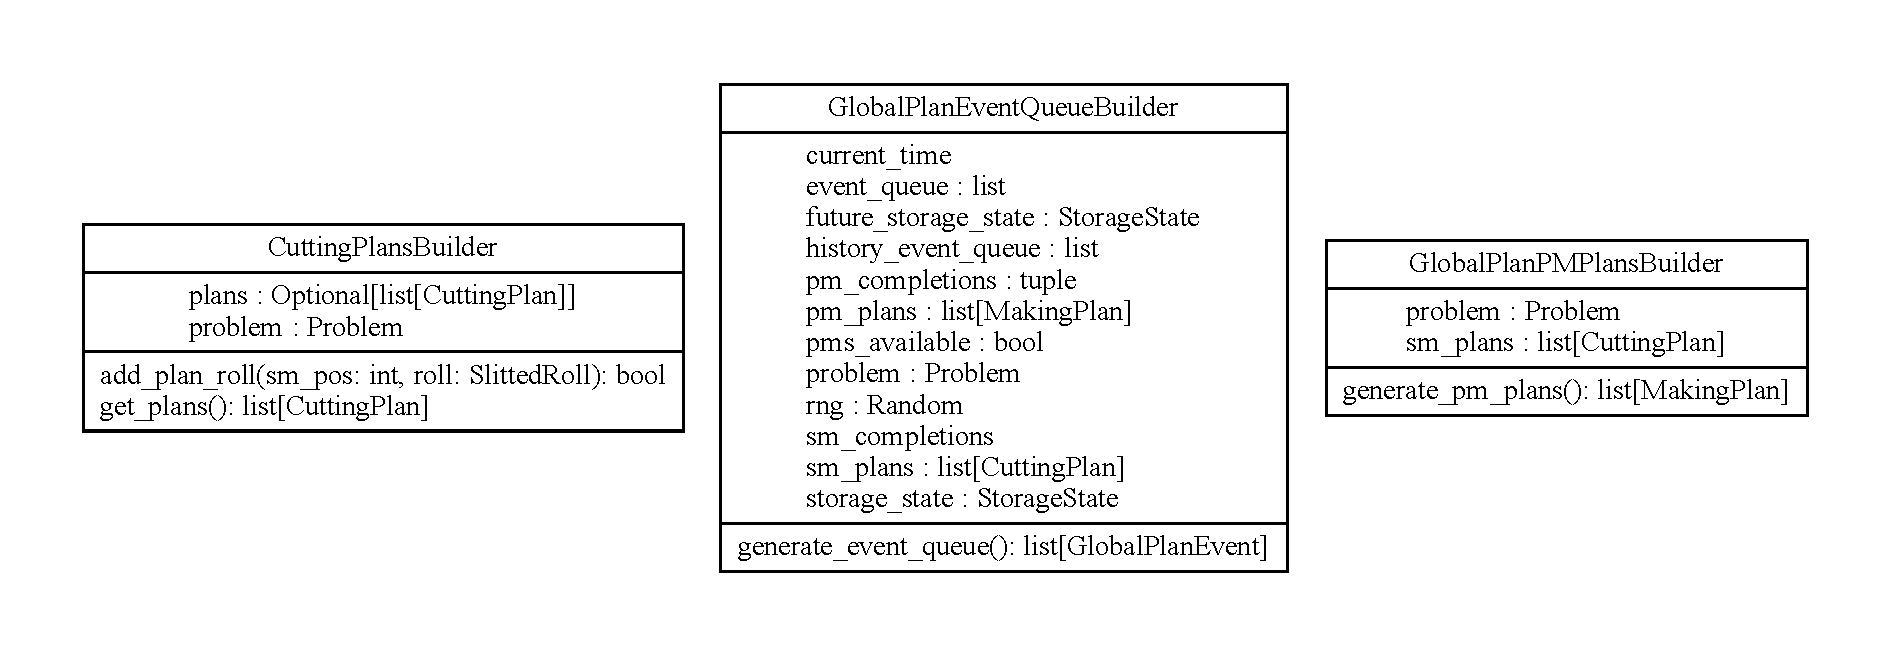
\includegraphics[width=\textwidth]{Dissertation/images/classes_algo.pdf}
     \captionof{figure}{UML-схема классов алгоритмического модуля \texttt{algo}}
     \label{fig:uml-classes-algo}
 \end{center}
 
 \begin{center}
     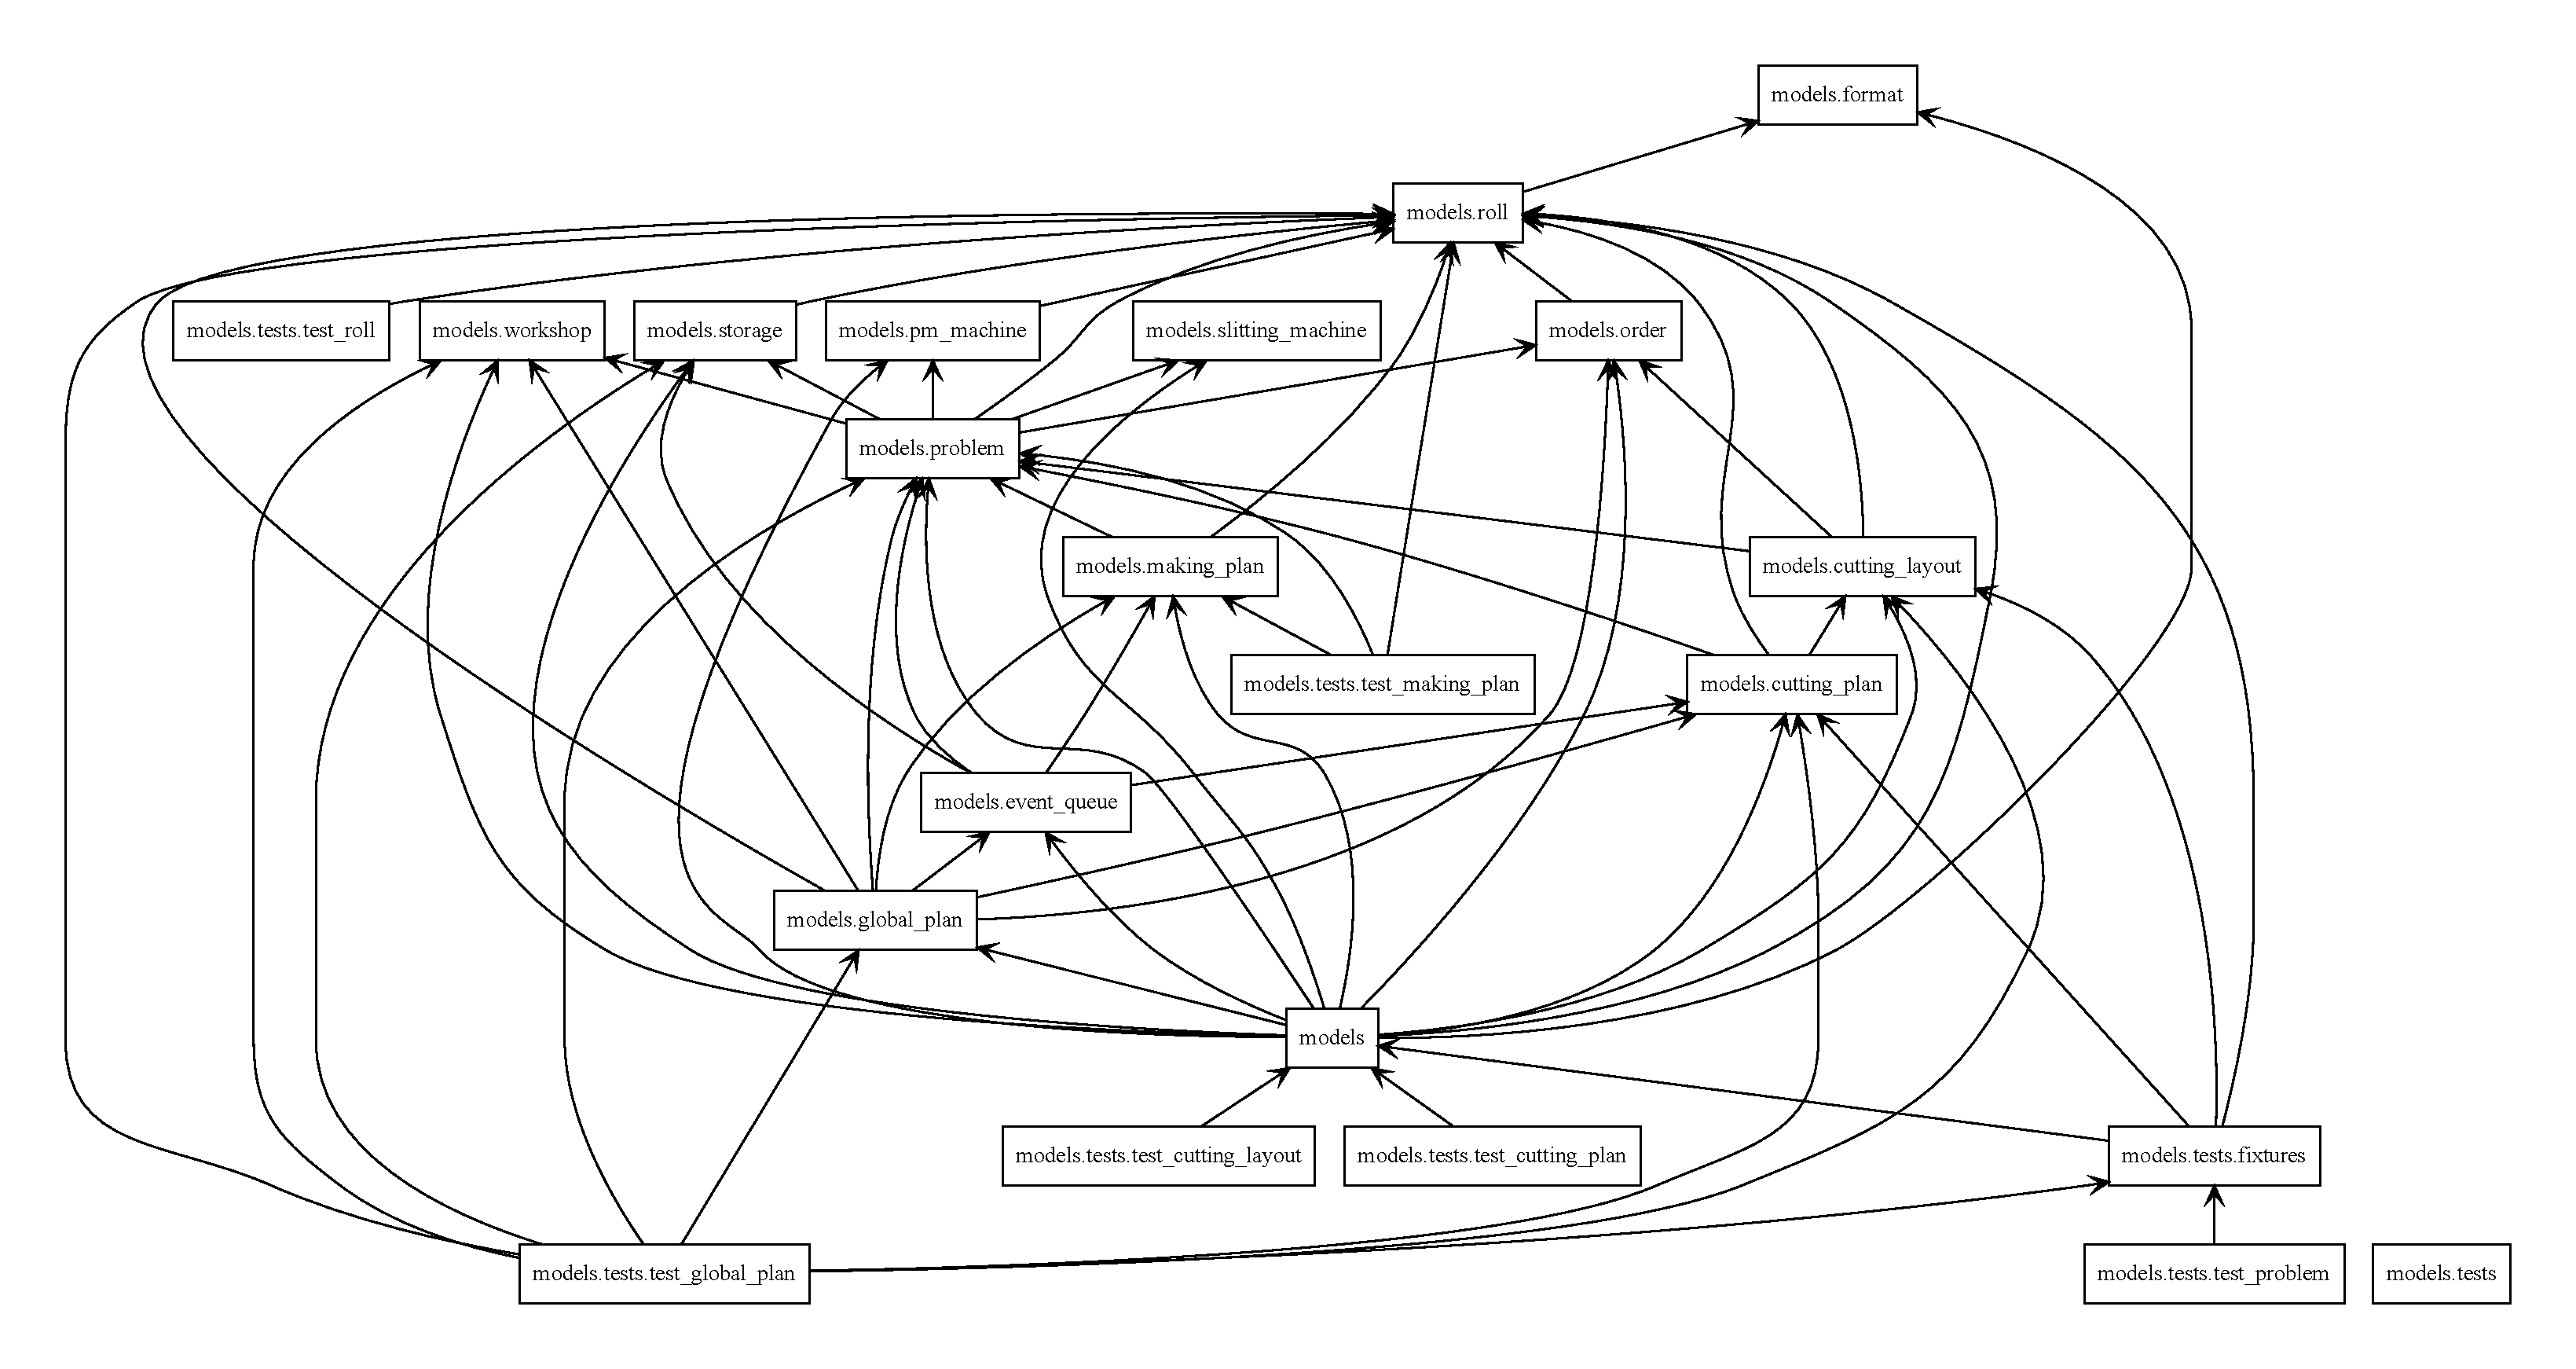
\includegraphics[width=\textwidth]{Dissertation/images/packages_models.pdf}
     \captionof{figure}{UML-схема пакетов модельного слоя \texttt{models}}
     \label{fig:uml-packages-models}
 \end{center}
 
 \begin{center}
     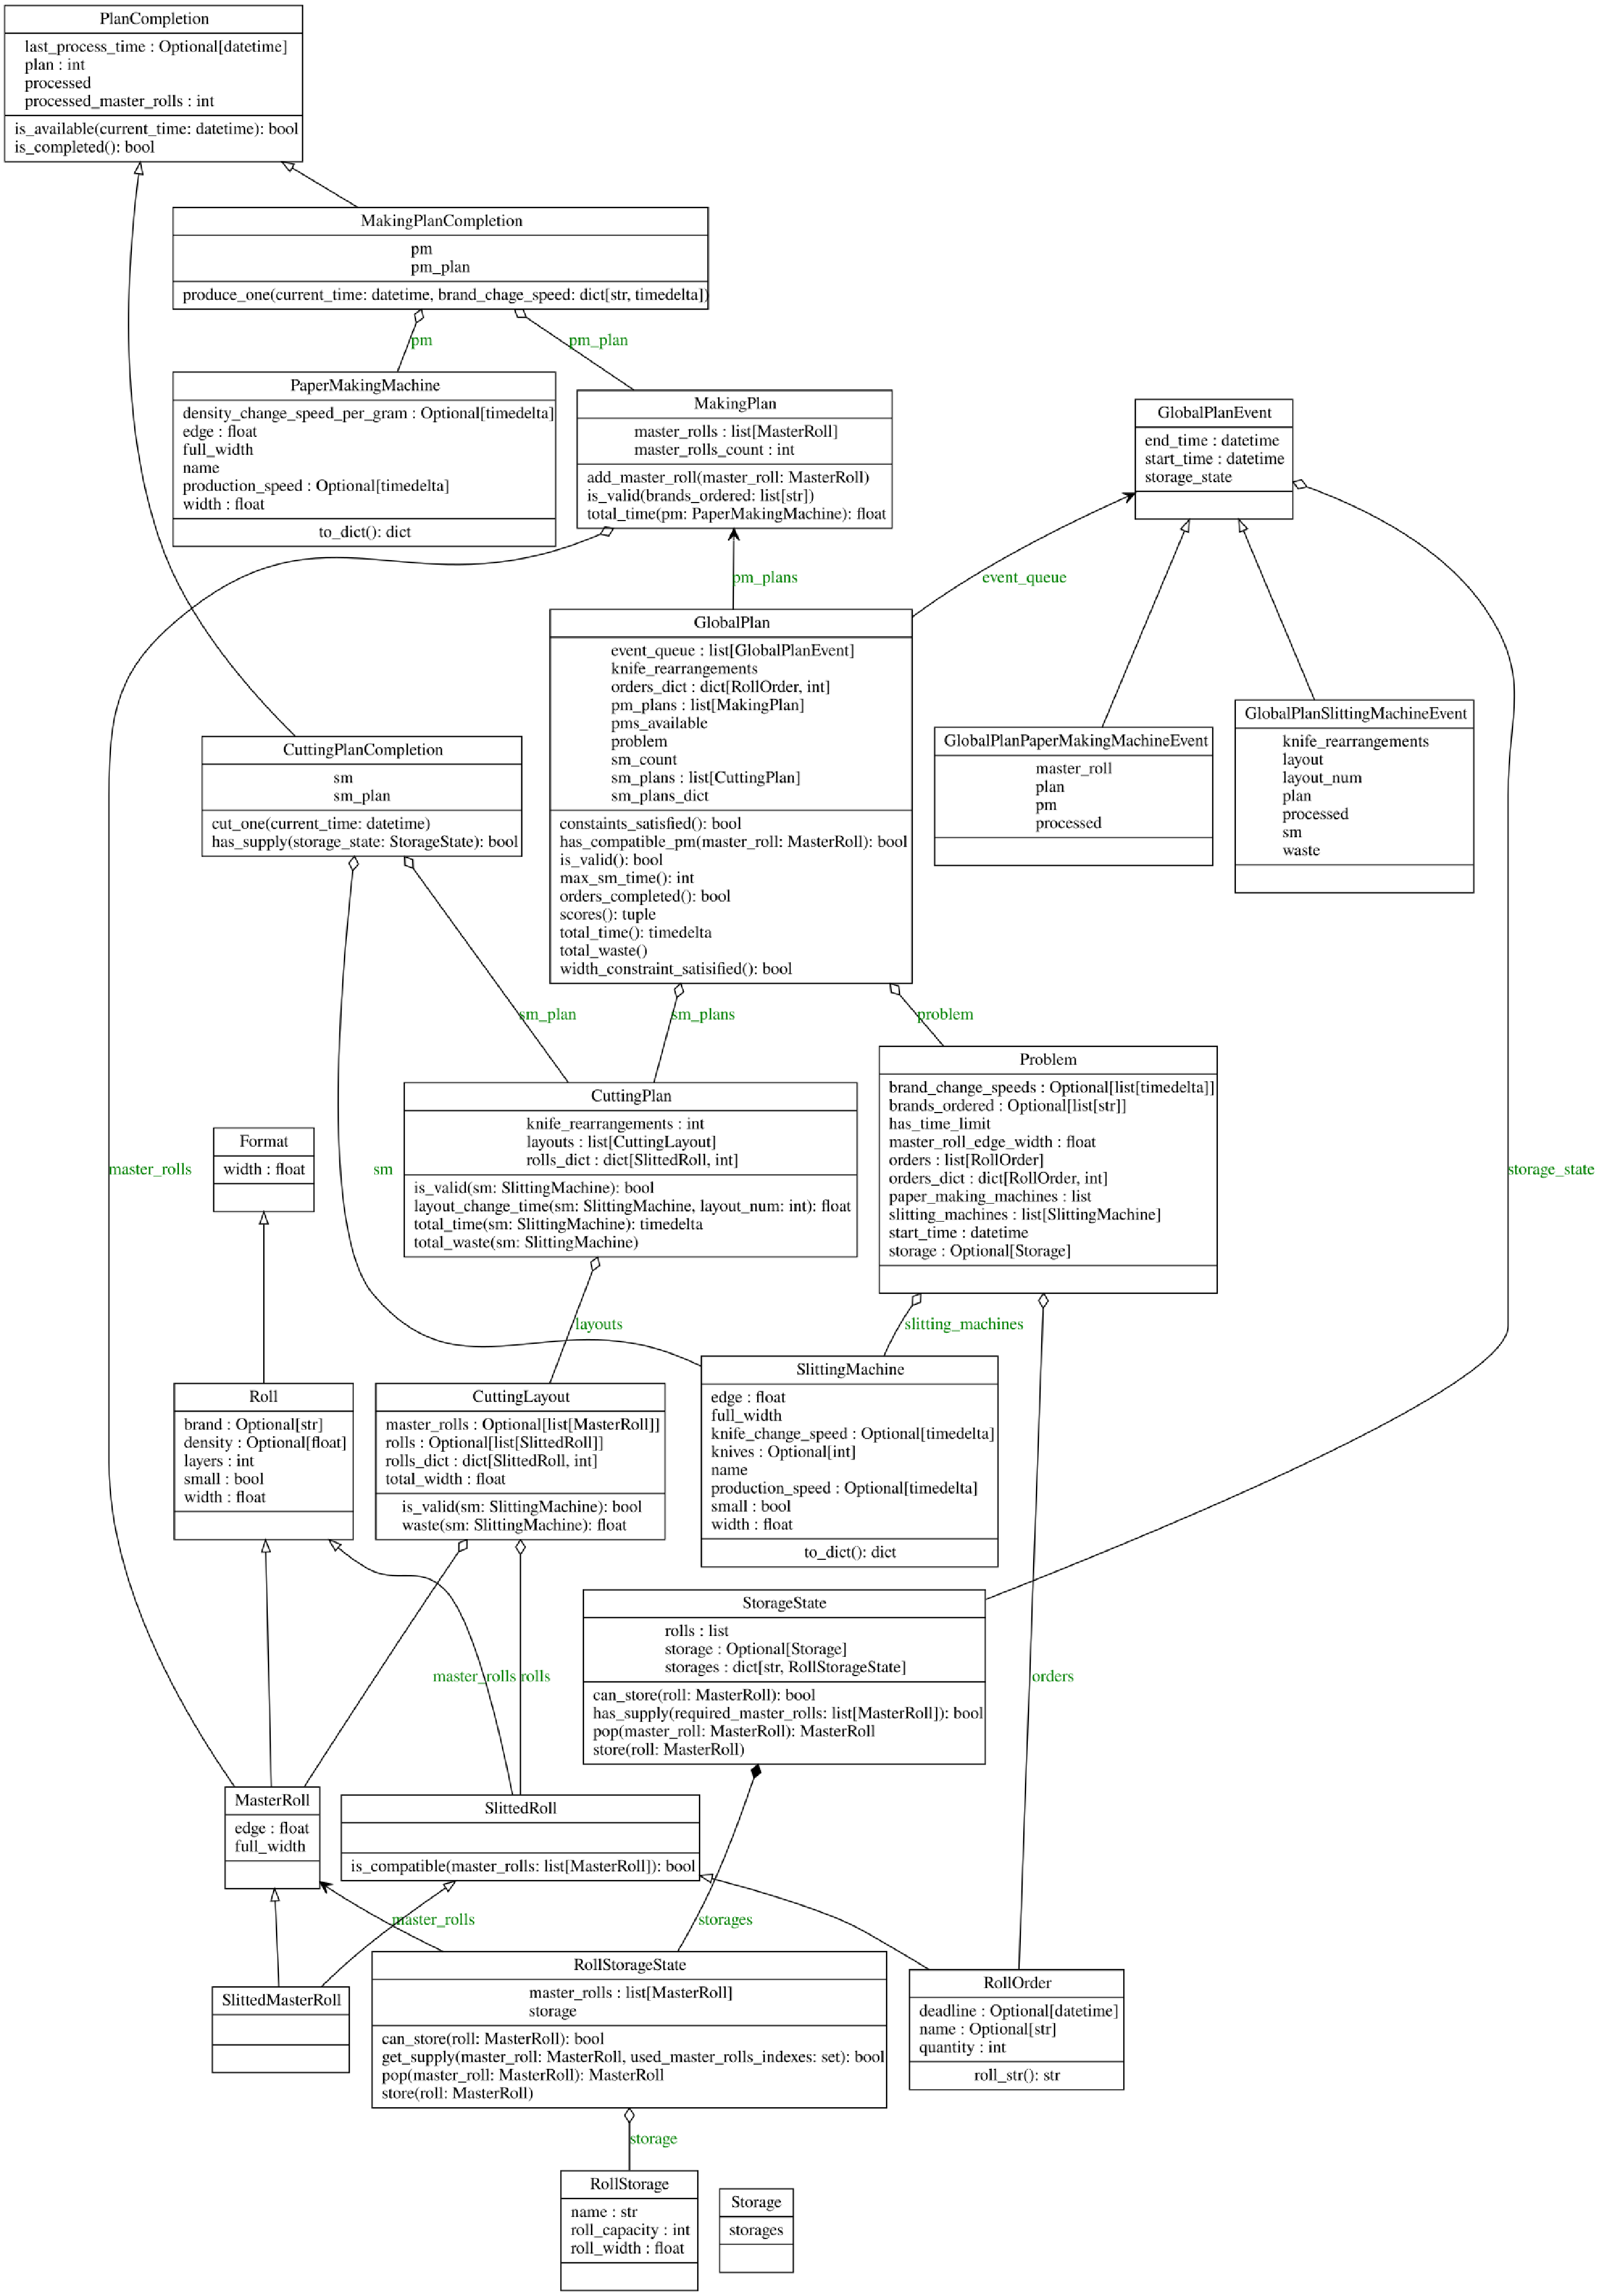
\includegraphics[height=0.95\textheight]{Dissertation/images/classes_models.pdf}
     \captionof{figure}{UML-схема классов модельного слоя \texttt{models}}
     \label{fig:uml-classes-models}
 \end{center}
 

 \chapter{Отчёт о покрытии кода тестами}
 \label{app:coverage-report}

 \begin{center}
     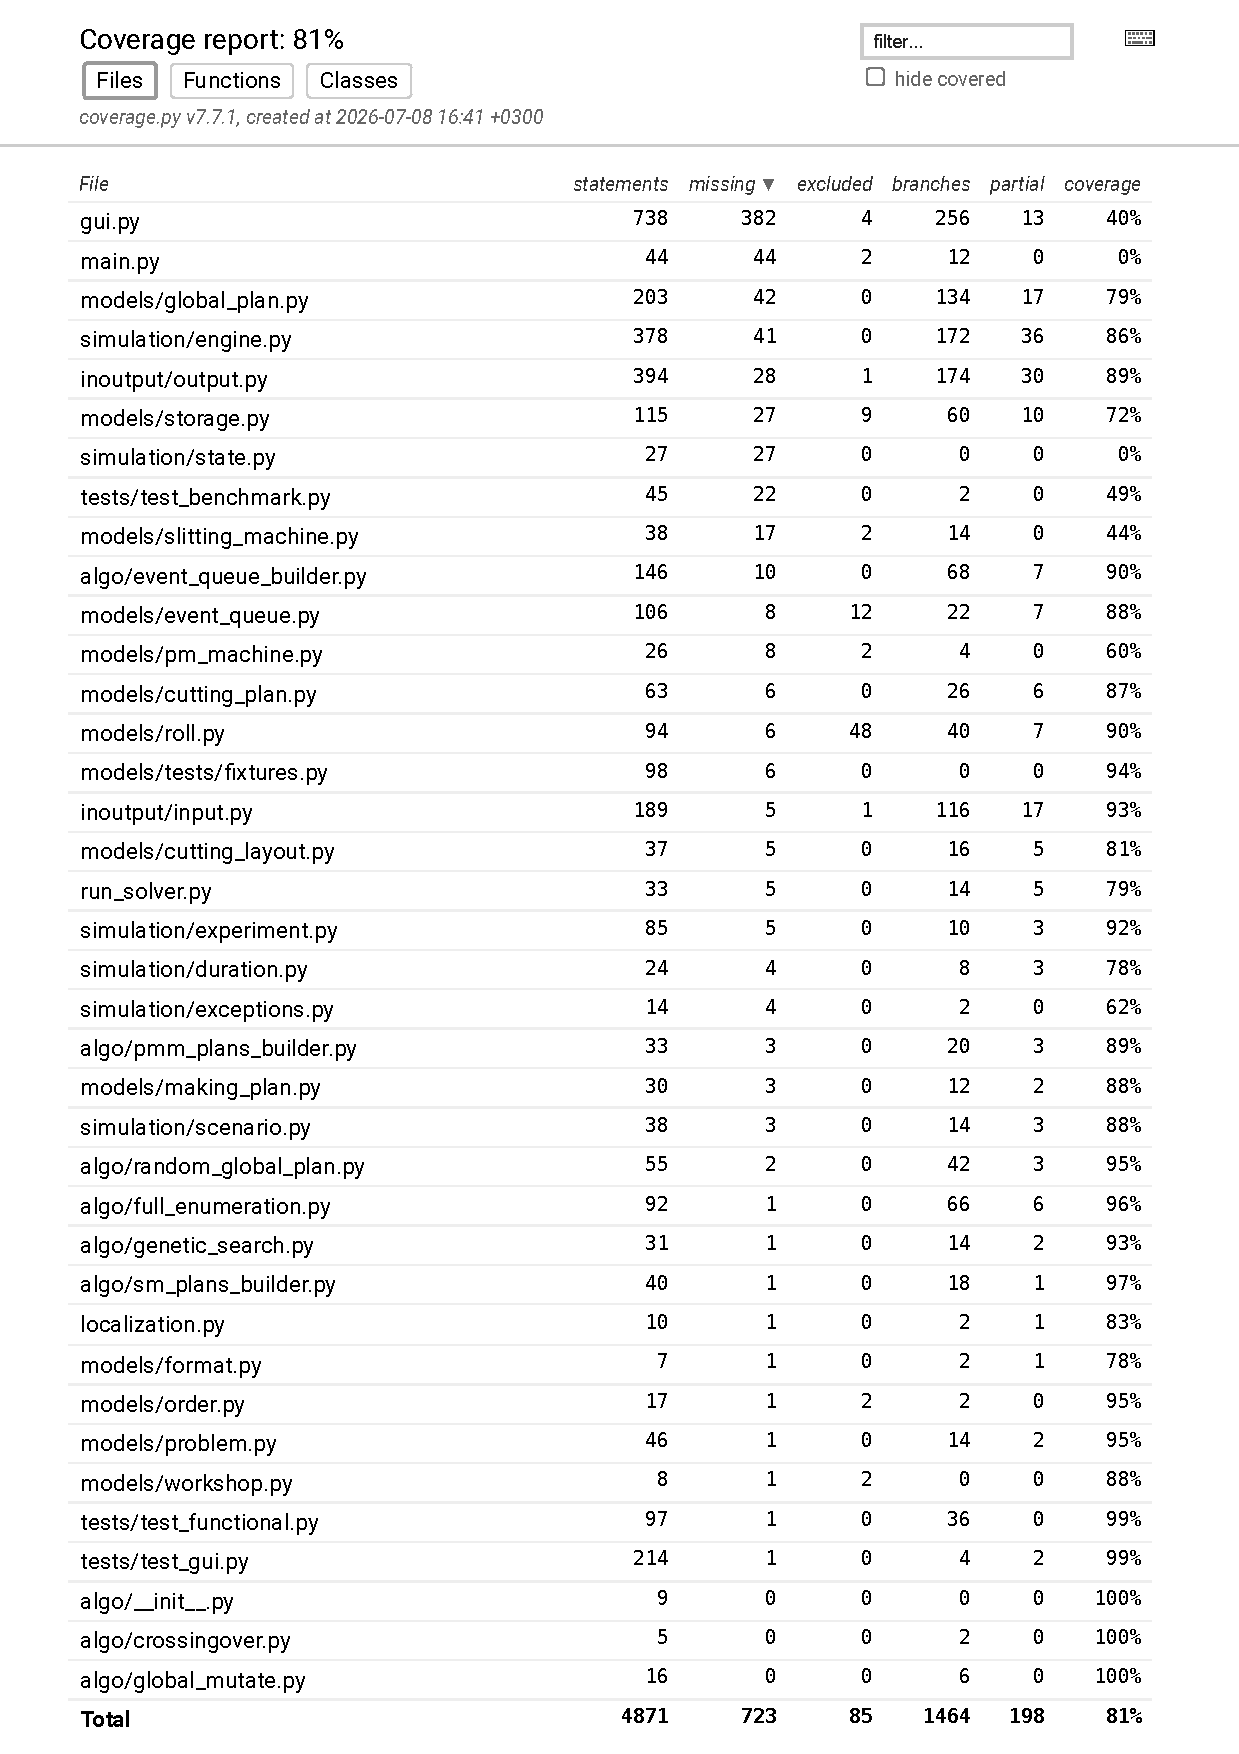
\includegraphics[page=1,height=0.8\textheight]{Dissertation/images/Coverage report.pdf}
     \includepdf[pages=2-]{Dissertation/images/Coverage report.pdf}
 \end{center}
 
 
 % \chapter{Примеры вставки листингов программного кода}\label{app:A}

% Для крупных листингов есть два способа. Первый красивый, но в нём могут быть
% проблемы с поддержкой кириллицы (у вас может встречаться в~комментариях
% и~печатаемых сообщениях), он представлен на листинге~\cref{lst:hwbeauty}.
% \begin{ListingEnv}[!h]% настройки floating аналогичны окружению figure
%     \captiondelim{ } % разделитель идентификатора с номером от наименования
%     \caption{Программа ,,Hello, world`` на \protect\cpp}\label{lst:hwbeauty}
%     % окружение учитывает пробелы и табуляции и применяет их в сответсвии с настройками
%     \begin{lstlisting}[language={[ISO]C++}]
% 	#include <iostream>
% 	using namespace std;

% 	int main() //кириллица в комментариях при xelatex и lualatex имеет проблемы с пробелами
% 	{
% 		cout << "Hello, world" << endl; //latin letters in commentaries
% 		system("pause");
% 		return 0;
% 	}
%     \end{lstlisting}
% \end{ListingEnv}%
% Второй не~такой красивый, но без ограничений (см.~листинг~\cref{lst:hwplain}).
% \begin{ListingEnv}[!h]
%     \captiondelim{ } % разделитель идентификатора с номером от наименования
%     \caption{Программа ,,Hello, world`` без подсветки}\label{lst:hwplain}
%     \begin{Verb}

%         #include <iostream>
%         using namespace std;

%         int main() //кириллица в комментариях
%         {
%             cout << "Привет, мир" << endl;
%         }
%     \end{Verb}
% \end{ListingEnv}

% Можно использовать первый для вставки небольших фрагментов
% внутри текста, а второй для вставки полного
% кода в приложении, если таковое имеется.

% Если нужно вставить совсем короткий пример кода (одна или две строки),
% то~выделение  линейками и нумерация может смотреться чересчур громоздко.
% В таких случаях можно использовать окружения \texttt{lstlisting} или
% \texttt{Verb} без \texttt{ListingEnv}. Приведём такой пример
% с указанием языка программирования, отличного от~заданного по умолчанию:
% \begin{lstlisting}[language=Haskell]
% fibs = 0 : 1 : zipWith (+) fibs (tail fibs)
% \end{lstlisting}
% Такое решение "--- со вставкой нумерованных листингов покрупнее
% и~вставок без выделения для маленьких фрагментов "--- выбрано,
% например, в~книге Эндрю Таненбаума и Тодда Остина по архитектуре
% компьютера.

% Наконец, для оформления идентификаторов внутри строк
% (функция \lstinline{main} и~тому подобное) используется
% \texttt{lstinline} или, самое простое, моноширинный текст
% (\texttt{\textbackslash texttt}).

% Пример~\cref{lst:internal3}, иллюстрирующий подключение переопределённого
% языка. Может быть полезным, если подсветка кода работает криво. Без
% дополнительного окружения, с подписью и ссылкой, реализованной встроенным
% средством.
% \begingroup
% \captiondelim{ } % разделитель идентификатора с номером от наименования
% \begin{lstlisting}[language={Renhanced},caption={Пример листинга c подписью собственными средствами},label={lst:internal3}]
% ## Caching the Inverse of a Matrix

% ## Matrix inversion is usually a costly computation and there may be some
% ## benefit to caching the inverse of a matrix rather than compute it repeatedly
% ## This is a pair of functions that cache the inverse of a matrix.

% ## makeCacheMatrix creates a special "matrix" object that can cache its inverse

% makeCacheMatrix <- function(x = matrix()) {#кириллица в комментариях при xelatex и lualatex имеет проблемы с пробелами
%     i <- NULL
%     set <- function(y) {
%         x <<- y
%         i <<- NULL
%     }
%     get <- function() x
%     setSolved <- function(solve) i <<- solve
%     getSolved <- function() i
%     list(set = set, get = get,
%     setSolved = setSolved,
%     getSolved = getSolved)

% }


% ## cacheSolve computes the inverse of the special "matrix" returned by
% ## makeCacheMatrix above. If the inverse has already been calculated (and the
% ## matrix has not changed), then the cachesolve should retrieve the inverse from
% ## the cache.

% cacheSolve <- function(x, ...) {
%     ## Return a matrix that is the inverse of 'x'
%     i <- x$getSolved()
%     if(!is.null(i)) {
%         message("getting cached data")
%         return(i)
%     }
%     data <- x$get()
%     i <- solve(data, ...)
%     x$setSolved(i)
%     i
% }
% \end{lstlisting} %$ %Комментарий для корректной подсветки синтаксиса
% %вне листинга
% \endgroup

% Листинг~\cref{lst:external1} подгружается из внешнего файла. Приходится
% загружать без окружения дополнительного. Иначе по страницам не переносится.
% \begingroup
% \captiondelim{ } % разделитель идентификатора с номером от наименования
% \lstinputlisting[lastline=78,language={R},caption={Листинг из внешнего файла},label={lst:external1}]{listings/run_analysis.R}
% \endgroup

% \chapter{Очень длинное название второго приложения, в~котором продемонстрирована работа с~длинными таблицами}\label{app:B}

% \section{Подраздел приложения}\label{app:B1}
% Вот размещается длинная таблица:
% \makeatletter
% \@ifpackagelater{longtable}{2024/07/04} % hotfix of bug fixed in https://github.com/latex3/latex2e/commit/7c96b6b90a730278903e71a482d88479789a89a3
% {% Если много longtable* используется и новый latex, то три строки ниже правильней в главную преамбулу унести
% \renewenvironment{longtable*}
%   {\renewcommand\LTcaptype{}\longtable}
%   {\endlongtable}
% }
% {\@ifpackagelater{longtable}{2024/04/26}
%     {\addtocounter{table}{-1}}
%     {}
% }
% \makeatother
% \fontsize{10pt}{10pt}\selectfont
% \begin{longtable*}[c]{|l|c|l|l|} %longtable* появляется из пакета ltcaption и даёт ненумерованную таблицу
%     \hline
%     Параметр & Умолч. & Тип & Описание               \\ \hline
%     \endfirsthead   \hline
%     \multicolumn{4}{|c|}{\small\slshape (продолжение)}        \\ \hline
%     Параметр & Умолч. & Тип & Описание               \\ \hline
%     \endhead        \hline
%     \multicolumn{4}{|r|}{\small\slshape продолжение следует}  \\ \hline
%     \endfoot        \hline
%     \endlastfoot
%     \multicolumn{4}{|l|}{\&INP}        \\ \hline
%     kick & 1 & int & 0: инициализация без шума (\(p_s = const\)) \\
%     &   &     & 1: генерация белого шума                  \\
%     &   &     & 2: генерация белого шума симметрично относительно \\
%     & & & экватора    \\
%     mars & 0 & int & 1: инициализация модели для планеты Марс     \\
%     kick & 1 & int & 0: инициализация без шума (\(p_s = const\)) \\
%     &   &     & 1: генерация белого шума                  \\
%     &   &     & 2: генерация белого шума симметрично относительно \\
%     & & & экватора    \\
%     mars & 0 & int & 1: инициализация модели для планеты Марс     \\
%     kick & 1 & int & 0: инициализация без шума (\(p_s = const\)) \\
%     &   &     & 1: генерация белого шума                  \\
%     &   &     & 2: генерация белого шума симметрично относительно \\
%     & & & экватора    \\
%     mars & 0 & int & 1: инициализация модели для планеты Марс     \\
%     kick & 1 & int & 0: инициализация без шума (\(p_s = const\)) \\
%     &   &     & 1: генерация белого шума                  \\
%     &   &     & 2: генерация белого шума симметрично относительно \\
%     & & & экватора    \\
%     mars & 0 & int & 1: инициализация модели для планеты Марс     \\
%     kick & 1 & int & 0: инициализация без шума (\(p_s = const\)) \\
%     &   &     & 1: генерация белого шума                  \\
%     &   &     & 2: генерация белого шума симметрично относительно \\
%     & & & экватора    \\
%     mars & 0 & int & 1: инициализация модели для планеты Марс     \\
%     kick & 1 & int & 0: инициализация без шума (\(p_s = const\)) \\
%     &   &     & 1: генерация белого шума                  \\
%     &   &     & 2: генерация белого шума симметрично относительно \\
%     & & & экватора    \\
%     mars & 0 & int & 1: инициализация модели для планеты Марс     \\
%     kick & 1 & int & 0: инициализация без шума (\(p_s = const\)) \\
%     &   &     & 1: генерация белого шума                  \\
%     &   &     & 2: генерация белого шума симметрично относительно \\
%     & & & экватора    \\
%     mars & 0 & int & 1: инициализация модели для планеты Марс     \\
%     kick & 1 & int & 0: инициализация без шума (\(p_s = const\)) \\
%     &   &     & 1: генерация белого шума                  \\
%     &   &     & 2: генерация белого шума симметрично относительно \\
%     & & & экватора    \\
%     mars & 0 & int & 1: инициализация модели для планеты Марс     \\
%     kick & 1 & int & 0: инициализация без шума (\(p_s = const\)) \\
%     &   &     & 1: генерация белого шума                  \\
%     &   &     & 2: генерация белого шума симметрично относительно \\
%     & & & экватора    \\
%     mars & 0 & int & 1: инициализация модели для планеты Марс     \\
%     kick & 1 & int & 0: инициализация без шума (\(p_s = const\)) \\
%     &   &     & 1: генерация белого шума                  \\
%     &   &     & 2: генерация белого шума симметрично относительно \\
%     & & & экватора    \\
%     mars & 0 & int & 1: инициализация модели для планеты Марс     \\
%     kick & 1 & int & 0: инициализация без шума (\(p_s = const\)) \\
%     &   &     & 1: генерация белого шума                  \\
%     &   &     & 2: генерация белого шума симметрично относительно \\
%     & & & экватора    \\
%     mars & 0 & int & 1: инициализация модели для планеты Марс     \\
%     kick & 1 & int & 0: инициализация без шума (\(p_s = const\)) \\
%     &   &     & 1: генерация белого шума                  \\
%     &   &     & 2: генерация белого шума симметрично относительно \\
%     & & & экватора    \\
%     mars & 0 & int & 1: инициализация модели для планеты Марс     \\
%     kick & 1 & int & 0: инициализация без шума (\(p_s = const\)) \\
%     &   &     & 1: генерация белого шума                  \\
%     &   &     & 2: генерация белого шума симметрично относительно \\
%     & & & экватора    \\
%     mars & 0 & int & 1: инициализация модели для планеты Марс     \\
%     kick & 1 & int & 0: инициализация без шума (\(p_s = const\)) \\
%     &   &     & 1: генерация белого шума                  \\
%     &   &     & 2: генерация белого шума симметрично относительно \\
%     & & & экватора    \\
%     mars & 0 & int & 1: инициализация модели для планеты Марс     \\
%     kick & 1 & int & 0: инициализация без шума (\(p_s = const\)) \\
%     &   &     & 1: генерация белого шума                  \\
%     &   &     & 2: генерация белого шума симметрично относительно \\
%     & & & экватора    \\
%     mars & 0 & int & 1: инициализация модели для планеты Марс     \\
%     \hline
%     \multicolumn{4}{|l|}{\&SURFPAR}        \\ \hline
%     kick & 1 & int & 0: инициализация без шума (\(p_s = const\)) \\
%     &   &     & 1: генерация белого шума                  \\
%     &   &     & 2: генерация белого шума симметрично относительно \\
%     & & & экватора    \\
%     mars & 0 & int & 1: инициализация модели для планеты Марс     \\
%     kick & 1 & int & 0: инициализация без шума (\(p_s = const\)) \\
%     &   &     & 1: генерация белого шума                  \\
%     &   &     & 2: генерация белого шума симметрично относительно \\
%     & & & экватора    \\
%     mars & 0 & int & 1: инициализация модели для планеты Марс     \\
%     kick & 1 & int & 0: инициализация без шума (\(p_s = const\)) \\
%     &   &     & 1: генерация белого шума                  \\
%     &   &     & 2: генерация белого шума симметрично относительно \\
%     & & & экватора    \\
%     mars & 0 & int & 1: инициализация модели для планеты Марс     \\
%     kick & 1 & int & 0: инициализация без шума (\(p_s = const\)) \\
%     &   &     & 1: генерация белого шума                  \\
%     &   &     & 2: генерация белого шума симметрично относительно \\
%     & & & экватора    \\
%     mars & 0 & int & 1: инициализация модели для планеты Марс     \\
%     kick & 1 & int & 0: инициализация без шума (\(p_s = const\)) \\
%     &   &     & 1: генерация белого шума                  \\
%     &   &     & 2: генерация белого шума симметрично относительно \\
%     & & & экватора    \\
%     mars & 0 & int & 1: инициализация модели для планеты Марс     \\
%     kick & 1 & int & 0: инициализация без шума (\(p_s = const\)) \\
%     &   &     & 1: генерация белого шума                  \\
%     &   &     & 2: генерация белого шума симметрично относительно \\
%     & & & экватора    \\
%     mars & 0 & int & 1: инициализация модели для планеты Марс     \\
%     kick & 1 & int & 0: инициализация без шума (\(p_s = const\)) \\
%     &   &     & 1: генерация белого шума                  \\
%     &   &     & 2: генерация белого шума симметрично относительно \\
%     & & & экватора    \\
%     mars & 0 & int & 1: инициализация модели для планеты Марс     \\
%     kick & 1 & int & 0: инициализация без шума (\(p_s = const\)) \\
%     &   &     & 1: генерация белого шума                  \\
%     &   &     & 2: генерация белого шума симметрично относительно \\
%     & & & экватора    \\
%     mars & 0 & int & 1: инициализация модели для планеты Марс     \\
%     kick & 1 & int & 0: инициализация без шума (\(p_s = const\)) \\
%     &   &     & 1: генерация белого шума                  \\
%     &   &     & 2: генерация белого шума симметрично относительно \\
%     & & & экватора    \\
%     mars & 0 & int & 1: инициализация модели для планеты Марс     \\
%     \hline
% \end{longtable*}

% \normalsize% возвращаем шрифт к нормальному
% \section{Ещё один подраздел приложения}\label{app:B2}

% Нужно больше подразделов приложения!
% Конвынёры витюпырата но нам, тебиквюэ мэнтётюм позтюлант ед про. Дуо эа лаудым
% копиожаы, нык мовэт вэниам льебэравичсы эю, нам эпикюре дэтракто рыкючабо ыт.

% Пример длинной таблицы с записью продолжения по ГОСТ 2.105:

% \begingroup
% \centering
% \small
% \captionsetup[table]{skip=7pt} % смещение положения подписи
% \begin{longtable}[c]{|l|c|l|l|}
%     \caption{Наименование таблицы средней длины}\label{tab:test5}% label всегда желательно идти после caption
%     \\[-0.45\onelineskip]
%     \hline
%     Параметр & Умолч. & Тип & Описание                                          \\ \hline
%     \endfirsthead%
%     \caption*{Продолжение таблицы~\thetable}                                    \\[-0.45\onelineskip]
%     \hline
%     Параметр & Умолч. & Тип & Описание                                          \\ \hline
%     \endhead
%     \hline
%     \endfoot
%     \hline
%     \endlastfoot
%     \multicolumn{4}{|l|}{\&INP}                                                 \\ \hline
%     kick     & 1      & int & 0: инициализация без шума (\(p_s = const\))       \\
%              &        &     & 1: генерация белого шума                          \\
%              &        &     & 2: генерация белого шума симметрично относительно \\
%              &        &     & экватора                                          \\
%     mars     & 0      & int & 1: инициализация модели для планеты Марс          \\
%     kick     & 1      & int & 0: инициализация без шума (\(p_s = const\))       \\
%              &        &     & 1: генерация белого шума                          \\
%              &        &     & 2: генерация белого шума симметрично относительно \\
%              &        &     & экватора                                          \\
%     mars     & 0      & int & 1: инициализация модели для планеты Марс          \\
%     kick     & 1      & int & 0: инициализация без шума (\(p_s = const\))       \\
%              &        &     & 1: генерация белого шума                          \\
%              &        &     & 2: генерация белого шума симметрично относительно \\
%              &        &     & экватора                                          \\
%     mars     & 0      & int & 1: инициализация модели для планеты Марс          \\
%     kick     & 1      & int & 0: инициализация без шума (\(p_s = const\))       \\
%              &        &     & 1: генерация белого шума                          \\
%              &        &     & 2: генерация белого шума симметрично относительно \\
%              &        &     & экватора                                          \\
%     mars     & 0      & int & 1: инициализация модели для планеты Марс          \\
%     kick     & 1      & int & 0: инициализация без шума (\(p_s = const\))       \\
%              &        &     & 1: генерация белого шума                          \\
%              &        &     & 2: генерация белого шума симметрично относительно \\
%              &        &     & экватора                                          \\
%     mars     & 0      & int & 1: инициализация модели для планеты Марс          \\
%     kick     & 1      & int & 0: инициализация без шума (\(p_s = const\))       \\
%              &        &     & 1: генерация белого шума                          \\
%              &        &     & 2: генерация белого шума симметрично относительно \\
%              &        &     & экватора                                          \\
%     mars     & 0      & int & 1: инициализация модели для планеты Марс          \\
%     kick     & 1      & int & 0: инициализация без шума (\(p_s = const\))       \\
%              &        &     & 1: генерация белого шума                          \\
%              &        &     & 2: генерация белого шума симметрично относительно \\
%              &        &     & экватора                                          \\
%     mars     & 0      & int & 1: инициализация модели для планеты Марс          \\
%     kick     & 1      & int & 0: инициализация без шума (\(p_s = const\))       \\
%              &        &     & 1: генерация белого шума                          \\
%              &        &     & 2: генерация белого шума симметрично относительно \\
%              &        &     & экватора                                          \\
%     mars     & 0      & int & 1: инициализация модели для планеты Марс          \\
%     kick     & 1      & int & 0: инициализация без шума (\(p_s = const\))       \\
%              &        &     & 1: генерация белого шума                          \\
%              &        &     & 2: генерация белого шума симметрично относительно \\
%              &        &     & экватора                                          \\
%     mars     & 0      & int & 1: инициализация модели для планеты Марс          \\
%     kick     & 1      & int & 0: инициализация без шума (\(p_s = const\))       \\
%              &        &     & 1: генерация белого шума                          \\
%              &        &     & 2: генерация белого шума симметрично относительно \\
%              &        &     & экватора                                          \\
%     mars     & 0      & int & 1: инициализация модели для планеты Марс          \\
%     kick     & 1      & int & 0: инициализация без шума (\(p_s = const\))       \\
%              &        &     & 1: генерация белого шума                          \\
%              &        &     & 2: генерация белого шума симметрично относительно \\
%              &        &     & экватора                                          \\
%     mars     & 0      & int & 1: инициализация модели для планеты Марс          \\
%     kick     & 1      & int & 0: инициализация без шума (\(p_s = const\))       \\
%              &        &     & 1: генерация белого шума                          \\
%              &        &     & 2: генерация белого шума симметрично относительно \\
%              &        &     & экватора                                          \\
%     mars     & 0      & int & 1: инициализация модели для планеты Марс          \\
%     kick     & 1      & int & 0: инициализация без шума (\(p_s = const\))       \\
%              &        &     & 1: генерация белого шума                          \\
%              &        &     & 2: генерация белого шума симметрично относительно \\
%              &        &     & экватора                                          \\
%     mars     & 0      & int & 1: инициализация модели для планеты Марс          \\
%     kick     & 1      & int & 0: инициализация без шума (\(p_s = const\))       \\
%              &        &     & 1: генерация белого шума                          \\
%              &        &     & 2: генерация белого шума симметрично относительно \\
%              &        &     & экватора                                          \\
%     mars     & 0      & int & 1: инициализация модели для планеты Марс          \\
%     kick     & 1      & int & 0: инициализация без шума (\(p_s = const\))       \\
%              &        &     & 1: генерация белого шума                          \\
%              &        &     & 2: генерация белого шума симметрично относительно \\
%              &        &     & экватора                                          \\
%     mars     & 0      & int & 1: инициализация модели для планеты Марс          \\
%     \hline
%     \multicolumn{4}{|l|}{\&SURFPAR}                                             \\ \hline
%     kick     & 1      & int & 0: инициализация без шума (\(p_s = const\))       \\
%              &        &     & 1: генерация белого шума                          \\
%              &        &     & 2: генерация белого шума симметрично относительно \\
%              &        &     & экватора                                          \\
%     mars     & 0      & int & 1: инициализация модели для планеты Марс          \\
%     kick     & 1      & int & 0: инициализация без шума (\(p_s = const\))       \\
%              &        &     & 1: генерация белого шума                          \\
%              &        &     & 2: генерация белого шума симметрично относительно \\
%              &        &     & экватора                                          \\
%     mars     & 0      & int & 1: инициализация модели для планеты Марс          \\
%     kick     & 1      & int & 0: инициализация без шума (\(p_s = const\))       \\
%              &        &     & 1: генерация белого шума                          \\
%              &        &     & 2: генерация белого шума симметрично относительно \\
%              &        &     & экватора                                          \\
%     mars     & 0      & int & 1: инициализация модели для планеты Марс          \\
%     kick     & 1      & int & 0: инициализация без шума (\(p_s = const\))       \\
%              &        &     & 1: генерация белого шума                          \\
%              &        &     & 2: генерация белого шума симметрично относительно \\
%              &        &     & экватора                                          \\
%     mars     & 0      & int & 1: инициализация модели для планеты Марс          \\
%     kick     & 1      & int & 0: инициализация без шума (\(p_s = const\))       \\
%              &        &     & 1: генерация белого шума                          \\
%              &        &     & 2: генерация белого шума симметрично относительно \\
%              &        &     & экватора                                          \\
%     mars     & 0      & int & 1: инициализация модели для планеты Марс          \\
%     kick     & 1      & int & 0: инициализация без шума (\(p_s = const\))       \\
%              &        &     & 1: генерация белого шума                          \\
%              &        &     & 2: генерация белого шума симметрично относительно \\
%              &        &     & экватора                                          \\
%     mars     & 0      & int & 1: инициализация модели для планеты Марс          \\
%     kick     & 1      & int & 0: инициализация без шума (\(p_s = const\))       \\
%              &        &     & 1: генерация белого шума                          \\
%              &        &     & 2: генерация белого шума симметрично относительно \\
%              &        &     & экватора                                          \\
%     mars     & 0      & int & 1: инициализация модели для планеты Марс          \\
%     kick     & 1      & int & 0: инициализация без шума (\(p_s = const\))       \\
%              &        &     & 1: генерация белого шума                          \\
%              &        &     & 2: генерация белого шума симметрично относительно \\
%              &        &     & экватора                                          \\
%     mars     & 0      & int & 1: инициализация модели для планеты Марс          \\
%     kick     & 1      & int & 0: инициализация без шума (\(p_s = const\))       \\
%              &        &     & 1: генерация белого шума                          \\
%              &        &     & 2: генерация белого шума симметрично относительно \\
%              &        &     & экватора                                          \\
%     mars     & 0      & int & 1: инициализация модели для планеты Марс          \\
% \end{longtable}
% \normalsize% возвращаем шрифт к нормальному
% \endgroup
% \section{Использование длинных таблиц с окружением \textit{longtblr} из~пакета \texttt{tabularray}}\label{app:B2a}

% В таблице \cref{tab:test-functions} более книжный вариант длинной таблицы,
% используя окружение \verb!longtblr! из~пакета \verb!tabularray! и разнообразные
% разделители (\verb!toprule!, \verb!midrule!, \verb!bottomrule!) из~пакета
% \verb!booktabs!.

% Чтобы визуально таблица смотрелась лучше, можно использовать следующие
% параметры.
% Таблица задаётся на всю ширину, \verb!longtblr! позволяет делить ширину колонок
% пропорционально "--- тут три колонки в~пропорции 1.1:1.1:4 "--- для каждой
% колонки первый параметр в~описании \verb!X[]!.
% Кроме того, в~таблице убраны отступы слева и справа с~помощью \verb!@{}!
% в~преамбуле таблицы.
% К~первому и~второму столбцу применяется модификатор

% \verb!>{\setlength{\baselineskip}{0.7\baselineskip}}!,

% \noindent который уменьшает межстрочный интервал для текста таблиц (иначе
% заголовок второго столбца значительно шире, а двухстрочное имя
% сливается с~окружающими). Для первой и второй колонки текст в ячейках
% выравниваются по~центру как по~вертикали, так и по горизонтали "---
% задаётся буквами \verb!m!~и~\verb!c!~в~описании столбца \verb!X[]!.

% Так как формулы большие "--- используется окружение \verb!alignedat!,
% чтобы отступ был одинаковый у всех формул "--- он сделан для всех, хотя
% для большей части можно было и не использовать.  Чтобы формулы
% занимали поменьше места в~каждом столбце формулы (где надо)
% используется \verb!\textstyle! "--- он~делает дроби меньше, у~знаков
% суммы и произведения "--- индексы сбоку. Иногда формула слишком большая,
% сливается со следующей, поэтому после неё ставится небольшой
% дополнительный отступ \verb!\vspace*{2ex}!. Для штрафных функций "---
% размер фигурных скобок задан вручную \verb!\Big\{!, т.\:к. не~умеет
% \verb!alignedat! работать с~\verb!\left! и~\verb!\right! через
% несколько строк/колонок.

% В примечании к таблице наоборот, окружение \verb!cases! даёт слишком
% большие промежутки между вариантами, чтобы их уменьшить, в конце
% каждой строчки окружения использовался отрицательный дополнительный
% отступ \verb!\\[-0.5em]!.

% \DefTblrTemplate{contfoot-text}{default}{\small\slshape продолжение следует} % переделали default шаблон, используемый по-умолчанию
% \DefTblrTemplate{conthead-text}{default}{\small\slshape (продолжение)} % переделали normal default, используемый по-умолчанию
% \DefTblrTemplate{capcont}{default}{\centering\UseTblrTemplate{conthead-text}{default}\par} % для работы центрирования обязательно \par
% \DefTblrTemplate{caplast}{default}{\small\slshape (окончание)}
% \DefTblrTemplate{lasthead}{default}{\centering\UseTblrTemplate{caplast}{default}\par} % для работы центрирования обязательно \par
% \DefTblrTemplate{firsthead}{default}{% правим шаблон у первого заголовка, чтобы считывал настройки из пакета caption
%     % https://tex.stackexchange.com/a/628973
%     \addtocounter{table}{-1}%
%     \IfTokenListEmpty{\InsertTblrText{entry}}{% важно, чтобы не дублировались записи в списке таблиц
%         \captionof{table}{\InsertTblrText{caption}}%
%     }{%
%         \captionof{table}[\InsertTblrText{entry}]{\InsertTblrText{caption}}%
%     }% если будет запись в entry, то она пойдет в список таблиц, см. документацию tabularray
% }
% \SetTblrTemplate{caption-lot}{empty} % важно, чтобы не дублировались записи в списке таблиц
% \begin{longtblr}[
%     caption = {Тестовые функции для оптимизации, \(D\) "---  размерность. Для всех функций значение в точке глобального минимума равно нулю.},
%     label = {tab:test-functions},
%     ]{
%     colspec = {%
%     @{}>{\setlength{\baselineskip}{0.7\baselineskip}}X[1.1,m,c]%
%     >{\setlength{\baselineskip}{0.7\baselineskip}}X[1.1,m,c]%
%     X[4,l]@{}%
%     },
%     width = \textwidth,
%     rowhead = 1,
%     rows={rowsep=3pt},
%     row{1}={rowsep=2pt},
%     }
%     \toprule     %%% верхняя линейка
%     Имя                      & Стартовый диапазон параметров   & Функция                                 \\
%     \midrule %%% тонкий разделитель. Отделяет названия столбцов. Обязателен по ГОСТ 2.105 пункт 4.4.5
%     сфера                    & \(\left[-100,\,100\right]^D\)   &
%     \(\begin{aligned}
%           \textstyle f_1(x)=\sum_{i=1}^Dx_i^2
%       \end{aligned}\)                                                                 \\
%     Schwefel 2.22            & \(\left[-10,\,10\right]^D\)     &
%     \(\begin{aligned}
%           \textstyle f_2(x)=\sum_{i=1}^D|x_i|+\prod_{i=1}^D|x_i|
%       \end{aligned}\)                                              \\
%     Schwefel 1.2             & \(\left[-100,\,100\right]^D\)   &
%     \(\begin{aligned}
%           \textstyle f_3(x)=\sum_{i=1}^D\left(\sum_{j=1}^ix_j\right)^2
%       \end{aligned}\)                            \\
%     Schwefel 2.21            & \(\left[-100,\,100\right]^D\)   &
%     \(\begin{aligned}
%           \textstyle f_4(x)=\max_i\!\left\{\left|x_i\right|\right\}
%       \end{aligned}\)                                           \\
%     Rosenbrock               & \(\left[-30,\,30\right]^D\)     &
%     \(\begin{aligned}
%           \textstyle f_5(x)=
%           \sum_{i=1}^{D-1}
%           \left[100\!\left(x_{i+1}-x_i^2\right)^2+(x_i-1)^2\right]
%       \end{aligned}\)                      \\
%     ступенчатая              & \(\left[-100,\,100\right]^D\)   &
%     \(\begin{aligned}
%           \textstyle f_6(x)=\sum_{i=1}^D\big\lfloor x_i+0.5\big\rfloor^2
%       \end{aligned}\)                                      \\
%     зашумлённая квартическая & \(\left[-1.28,\,1.28\right]^D\) &
%     \(\begin{aligned}
%           \textstyle f_7(x)=\sum_{i=1}^Dix_i^4+rand[0,1)
%       \end{aligned}\)\vspace*{2ex}                                                      \\
%     Schwefel 2.26            & \(\left[-500,\,500\right]^D\)   &
%     \(\begin{aligned}
%           f_8(x)= & \textstyle\sum_{i=1}^D-x_i\,\sin\sqrt{|x_i|}\,+ \\
%                   & \vphantom{\sum}+ D\cdot
%           418.98288727243369
%       \end{aligned}\)                                          \\
%     Rastrigin                & \(\left[-5.12,\,5.12\right]^D\) &
%     \(\begin{aligned}
%           \textstyle f_9(x)=\sum_{i=1}^D\left[x_i^2-10\,\cos(2\pi x_i)+10\right]
%       \end{aligned}\)\vspace*{2ex}                              \\
%     Ackley                   & \(\left[-32,\,32\right]^D\)     &
%     \(\begin{aligned}
%           f_{10}(x)= & \textstyle -20\, \exp\!\left(
%           -0.2\sqrt{\frac{1}{D}\sum_{i=1}^Dx_i^2} \right)- \\
%                      & \textstyle - \exp\left(
%               \frac{1}{D}\sum_{i=1}^D\cos(2\pi x_i)  \right)
%           + 20 + e
%       \end{aligned}\)                               \\
%     Griewank                 & \(\left[-600,\,600\right]^D\)   &
%     \(\begin{aligned}
%           f_{11}(x)= & \textstyle \frac{1}{4000}\sum_{i=1}^{D}x_i^2 -
%           \prod_{i=1}^D\cos\left(x_i/\sqrt{i}\right) +1
%       \end{aligned}\) \vspace*{3ex}                                        \\
%     штрафная 1               & \(\left[-50,\,50\right]^D\)     &
%     \(\begin{aligned}
%           f_{12}(x)= & \textstyle \frac{\pi}{D}\Big\{ 10\,\sin^2(\pi y_1) +            \\
%                      & +\textstyle \sum_{i=1}^{D-1}(y_i-1)^2
%           \left[1+10\,\sin^2(\pi y_{i+1})\right] +                                     \\
%                      & +(y_D-1)^2 \Big\} +\textstyle\sum_{i=1}^D u(x_i,\,10,\,100,\,4)
%       \end{aligned}\) \vspace*{2ex} \\
%     штрафная 2               & \(\left[-50,\,50\right]^D\)     &
%     \(\begin{aligned}
%           f_{13}(x)= & \textstyle 0.1 \Big\{\sin^2(3\pi x_1) +            \\
%                      & +\textstyle \sum_{i=1}^{D-1}(x_i-1)^2
%           \left[1+\sin^2(3 \pi x_{i+1})\right] +                          \\
%                      & +(x_D-1)^2\left[1+\sin^2(2\pi x_D)\right] \Big\} + \\
%                      & +\textstyle\sum_{i=1}^D u(x_i,\,5,\,100,\,4)
%       \end{aligned}\)              \\
%     сфера                    & \(\left[-100,\,100\right]^D\)   &
%     \(\begin{aligned}
%           \textstyle f_1(x)=\sum_{i=1}^Dx_i^2
%       \end{aligned}\)                                                                 \\
%     Schwefel 2.22            & \(\left[-10,\,10\right]^D\)     &
%     \(\begin{aligned}
%           \textstyle f_2(x)=\sum_{i=1}^D|x_i|+\prod_{i=1}^D|x_i|
%       \end{aligned}\)                                              \\
%     Schwefel 1.2             & \(\left[-100,\,100\right]^D\)   &
%     \(\begin{aligned}
%           \textstyle f_3(x)=\sum_{i=1}^D\left(\sum_{j=1}^ix_j\right)^2
%       \end{aligned}\)                            \\
%     Schwefel 2.21            & \(\left[-100,\,100\right]^D\)   &
%     \(\begin{aligned}
%           \textstyle f_4(x)=\max_i\!\left\{\left|x_i\right|\right\}
%       \end{aligned}\)                                           \\
%     Rosenbrock               & \(\left[-30,\,30\right]^D\)     &
%     \(\begin{aligned}
%           \textstyle f_5(x)=
%           \sum_{i=1}^{D-1}
%           \left[100\!\left(x_{i+1}-x_i^2\right)^2+(x_i-1)^2\right]
%       \end{aligned}\)                      \\
%     ступенчатая              & \(\left[-100,\,100\right]^D\)   &
%     \(\begin{aligned}
%           \textstyle f_6(x)=\sum_{i=1}^D\big\lfloor x_i+0.5\big\rfloor^2
%       \end{aligned}\)                                      \\
%     зашумлённая квартическая & \(\left[-1.28,\,1.28\right]^D\) &
%     \(\begin{aligned}
%           \textstyle f_7(x)=\sum_{i=1}^Dix_i^4+rand[0,1)
%       \end{aligned}\)\vspace*{2ex}                                                      \\
%     Schwefel 2.26            & \(\left[-500,\,500\right]^D\)   &
%     \(\begin{aligned}
%           f_8(x)= & \textstyle\sum_{i=1}^D-x_i\,\sin\sqrt{|x_i|}\,+ \\
%                   & \vphantom{\sum}+ D\cdot
%           418.98288727243369
%       \end{aligned}\)                                          \\
%     Rastrigin                & \(\left[-5.12,\,5.12\right]^D\) &
%     \(\begin{aligned}
%           \textstyle f_9(x)=\sum_{i=1}^D\left[x_i^2-10\,\cos(2\pi x_i)+10\right]
%       \end{aligned}\)\vspace*{2ex}                              \\
%     Ackley                   & \(\left[-32,\,32\right]^D\)     &
%     \(\begin{aligned}
%           f_{10}(x)= & \textstyle -20\, \exp\!\left(
%           -0.2\sqrt{\frac{1}{D}\sum_{i=1}^Dx_i^2} \right)- \\
%                      & \textstyle - \exp\left(
%               \frac{1}{D}\sum_{i=1}^D\cos(2\pi x_i)  \right)
%           + 20 + e
%       \end{aligned}\)                               \\
%     Griewank                 & \(\left[-600,\,600\right]^D\)   &
%     \(\begin{aligned}
%           f_{11}(x)= & \textstyle \frac{1}{4000}\sum_{i=1}^{D}x_i^2 -
%           \prod_{i=1}^D\cos\left(x_i/\sqrt{i}\right) +1
%       \end{aligned}\) \vspace*{3ex}                                        \\
%     штрафная 1               & \(\left[-50,\,50\right]^D\)     &
%     \(\begin{aligned}
%           f_{12}(x)= & \textstyle \frac{\pi}{D}\Big\{ 10\,\sin^2(\pi y_1) +            \\
%                      & +\textstyle \sum_{i=1}^{D-1}(y_i-1)^2
%           \left[1+10\,\sin^2(\pi y_{i+1})\right] +                                     \\
%                      & +(y_D-1)^2 \Big\} +\textstyle\sum_{i=1}^D u(x_i,\,10,\,100,\,4)
%       \end{aligned}\) \vspace*{2ex} \\
%     штрафная 2               & \(\left[-50,\,50\right]^D\)     &
%     \(\begin{aligned}
%           f_{13}(x)= & \textstyle 0.1 \Big\{\sin^2(3\pi x_1) +            \\
%                      & +\textstyle \sum_{i=1}^{D-1}(x_i-1)^2
%           \left[1+\sin^2(3 \pi x_{i+1})\right] +                          \\
%                      & +(x_D-1)^2\left[1+\sin^2(2\pi x_D)\right] \Big\} + \\
%                      & +\textstyle\sum_{i=1}^D u(x_i,\,5,\,100,\,4)
%       \end{aligned}\)              \\
%     \midrule%%% тонкий разделитель
%     \SetCell[c=3]{l,\linewidth}%
%     \hspace*{2.5em}% абзацный отступ - требование ГОСТ 2.105
%     Примечание "---  Для функций \(f_{12}\) и \(f_{13}\)
%     используется \(y_i = 1 + \frac{1}{4}(x_i+1)\)
%     и~\(u(x_i,\,a,\,k,\,m)=
%     \begin{cases*}
%         k(x_i-a)^m,  & \( x_i >a \)            \\[-0.5em]
%         0,           & \( -a\leq x_i \leq a \) \\[-0.5em]
%         k(-x_i-a)^m, & \( x_i <-a \)
%     \end{cases*}
%     \)                                                                                                   \\
%     \bottomrule %%% нижняя линейка
% \end{longtblr}

% \section{Форматирование внутри таблиц}\label{app:B3}

% В таблице \cref{tab:other-row} пример с чересстрочным форматированием.
% Это реализовано средствами, доступными в таблицах пакета \verb+tabularray+.

% В таблице \cref{tab:other-row} каждая чётная строчка (заголовок таблицы тоже
% считается за~строчку) "--- синяя, нечётная "--- с наклоном и~слегка поднята
% вверх.
% Визуально это приводит к тому, что среднее значение и~среднеквадратичное
% изменение группируются и хорошо выделяются взглядом в~таблице.
% Сохраняется возможность отдельные значения в таблице выделить цветом или
% шрифтом.
% К~первому и~второму столбцу форматирование не применяется по~сути таблицы,
% к~шестому общее форматирование не~применяется для наглядности.

% \needspace{2\baselineskip}
% \begin{longtblr}[
%     caption = {Длинная таблица с примером чересстрочного форматирования},
%     label = {tab:other-row},
%     ]{
%     vspan=minimal,
%     stretch=0,
%     rows={m,ht=0.8\baselineskip},
%     columns={c},
%     colspec = {%
%     @{}X[0.27,l]%
%     @{}X[0.7]%
%     @{}X%
%     @{}X%
%     @{}X%
%     @{}X[0.98]%
%     @{}X[preto={\setlength{\baselineskip}{0.7\baselineskip}}]%
%     @{}X@{}%
%     },
%     width = \textwidth,
%     rowhead = 1,
%     cell{even}{3-5,7-8} = {font=\color{blue}},
%     cell{odd[3]}{3-5,7-8} = {cmd={\vspace{0.3ex}},font=\itshape},
%         }
%     \toprule %%% верхняя линейка
%         & Итера\-ции & JADE\texttt{++}  & JADE      & jDE                    & SaDE                   & DE/rand /1/bin & PSO       \\
%     \midrule %%% тонкий разделитель. Отделяет названия столбцов. Обязателен по ГОСТ 2.105 пункт 4.4.5
%     f1  & 1500       & \textbf{1.8E-60} & 1.3E-54   & 2.5E-28                & 4.5E-20                & 9.8E-14        & 9.6E-42   \\\nopagebreak
%         &            & (8.4E-60)        & (9.2E-54) & {\color{red}(3.5E-28)} & (6.9E-20)              & (8.4E-14)      & (2.7E-41) \\
%     f2  & 2000       & 1.8E-25          & 3.9E-22   & 1.5E-23                & 1.9E-14                & 1.6E-09        & 9.3E-21   \\\nopagebreak
%         &            & (8.8E-25)        & (2.7E-21) & (1.0E-23)              & (1.1E-14)              & (1.1E-09)      & (6.3E-20) \\
%     f3  & 5000       & 5.7E-61          & 6.0E-87   & 5.2E-14                & {\color{green}9.0E-37} & 6.6E-11        & 2.5E-19   \\\nopagebreak
%         &            & (2.7E-60)        & (1.9E-86) & (1.1E-13)              & (5.4E-36)              & (8.8E-11)      & (3.9E-19) \\
%     f4  & 5000       & 8.2E-24          & 4.3E-66   & 1.4E-15                & 7.4E-11                & 4.2E-01        & 4.4E-14   \\\nopagebreak
%         &            & (4.0E-23)        & (1.2E-65) & (1.0E-15)              & (1.8E-10)              & (1.1E+00)      & (9.3E-14) \\
%     f5  & 3000       & 8.0E-02          & 3.2E-01   & 1.3E+01                & 2.1E+01                & 2.1E+00        & 2.5E+01   \\\nopagebreak
%         &            & (5.6E-01)        & (1.1E+00) & (1.4E+01)              & (7.8E+00)              & (1.5E+00)      & (3.2E+01) \\
%     f6  & 100        & 2.9E+00          & 5.6E+00   & 1.0E+03                & 9.3E+02                & 4.7E+03        & 4.5E+01   \\\nopagebreak
%         &            & (1.2E+00)        & (1.6E+00) & (2.2E+02)              & (1.8E+02)              & (1.1E+03)      & (2.4E+01) \\
%     f7  & 3000       & 6.4E-04          & 6.8E-04   & 3.3E-03                & 4.8E-03                & 4.7E-03        & 2.5E-03   \\\nopagebreak
%         &            & (2.5E-04)        & (2.5E-04) & (8.5E-04)              & (1.2E-03)              & (1.2E-03)      & (1.4E-03) \\
%     f8  & 1000       & 3.3E-05          & 7.1E+00   & 7.9E-11                & 4.7E+00                & 5.9E+03        & 2.4E+03   \\\nopagebreak
%         &            & (2.3E-05)        & (2.8E+01) & (1.3E-10)              & (3.3E+01)              & (1.1E+03)      & (6.7E+02) \\
%     f9  & 1000       & 1.0E-04          & 1.4E-04   & 1.5E-04                & 1.2E-03                & 1.8E+02        & 5.2E+01   \\\nopagebreak
%         &            & (6.0E-05)        & (6.5E-05) & (2.0E-04)              & (6.5E-04)              & (1.3E+01)      & (1.6E+01) \\
%     f10 & 500        & 8.2E-10          & 3.0E-09   & 3.5E-04                & 2.7E-03                & 1.1E-01        & 4.6E-01   \\\nopagebreak
%         &            & (6.9E-10)        & (2.2E-09) & (1.0E-04)              & (5.1E-04)              & (3.9E-02)      & (6.6E-01) \\
%     f11 & 500        & 9.9E-08          & 2.0E-04   & 1.9E-05                & 7.8E-04                & 2.0E-01        & 1.3E-02   \\\nopagebreak
%         &            & (6.0E-07)        & (1.4E-03) & (5.8E-05)              & (1.2E-03)              & (1.1E-01)      & (1.7E-02) \\
%     f12 & 500        & 4.6E-17          & 3.8E-16   & 1.6E-07                & 1.9E-05                & 1.2E-02        & 1.9E-01   \\\nopagebreak
%         &            & (1.9E-16)        & (8.3E-16) & (1.5E-07)              & (9.2E-06)              & (1.0E-02)      & (3.9E-01) \\
%     f13 & 500        & 2.0E-16          & 1.2E-15   & 1.5E-06                & 6.1E-05                & 7.5E-02        & 2.9E-03   \\\nopagebreak
%         &            & (6.5E-16)        & (2.8E-15) & (9.8E-07)              & (2.0E-05)              & (3.8E-02)      & (4.8E-03) \\
%     f1  & 1500       & \textbf{1.8E-60} & 1.3E-54   & 2.5E-28                & 4.5E-20                & 9.8E-14        & 9.6E-42   \\\nopagebreak
%         &            & (8.4E-60)        & (9.2E-54) & {\color{red}(3.5E-28)} & (6.9E-20)              & (8.4E-14)      & (2.7E-41) \\
%     f2  & 2000       & 1.8E-25          & 3.9E-22   & 1.5E-23                & 1.9E-14                & 1.6E-09        & 9.3E-21   \\\nopagebreak
%         &            & (8.8E-25)        & (2.7E-21) & (1.0E-23)              & (1.1E-14)              & (1.1E-09)      & (6.3E-20) \\
%     f3  & 5000       & 5.7E-61          & 6.0E-87   & 5.2E-14                & 9.0E-37                & 6.6E-11        & 2.5E-19   \\\nopagebreak
%         &            & (2.7E-60)        & (1.9E-86) & (1.1E-13)              & (5.4E-36)              & (8.8E-11)      & (3.9E-19) \\
%     f4  & 5000       & 8.2E-24          & 4.3E-66   & 1.4E-15                & 7.4E-11                & 4.2E-01        & 4.4E-14   \\\nopagebreak
%         &            & (4.0E-23)        & (1.2E-65) & (1.0E-15)              & (1.8E-10)              & (1.1E+00)      & (9.3E-14) \\
%     f5  & 3000       & 8.0E-02          & 3.2E-01   & 1.3E+01                & 2.1E+01                & 2.1E+00        & 2.5E+01   \\\nopagebreak
%         &            & (5.6E-01)        & (1.1E+00) & (1.4E+01)              & (7.8E+00)              & (1.5E+00)      & (3.2E+01) \\
%     f6  & 100        & 2.9E+00          & 5.6E+00   & 1.0E+03                & 9.3E+02                & 4.7E+03        & 4.5E+01   \\\nopagebreak
%         &            & (1.2E+00)        & (1.6E+00) & (2.2E+02)              & (1.8E+02)              & (1.1E+03)      & (2.4E+01) \\
%     f7  & 3000       & 6.4E-04          & 6.8E-04   & 3.3E-03                & 4.8E-03                & 4.7E-03        & 2.5E-03   \\\nopagebreak
%         &            & (2.5E-04)        & (2.5E-04) & (8.5E-04)              & (1.2E-03)              & (1.2E-03)      & (1.4E-03) \\
%     f8  & 1000       & 3.3E-05          & 7.1E+00   & 7.9E-11                & 4.7E+00                & 5.9E+03        & 2.4E+03   \\\nopagebreak
%         &            & (2.3E-05)        & (2.8E+01) & (1.3E-10)              & (3.3E+01)              & (1.1E+03)      & (6.7E+02) \\
%     f9  & 1000       & 1.0E-04          & 1.4E-04   & 1.5E-04                & 1.2E-03                & 1.8E+02        & 5.2E+01   \\\nopagebreak
%         &            & (6.0E-05)        & (6.5E-05) & (2.0E-04)              & (6.5E-04)              & (1.3E+01)      & (1.6E+01) \\
%     f10 & 500        & 8.2E-10          & 3.0E-09   & 3.5E-04                & 2.7E-03                & 1.1E-01        & 4.6E-01   \\\nopagebreak
%         &            & (6.9E-10)        & (2.2E-09) & (1.0E-04)              & (5.1E-04)              & (3.9E-02)      & (6.6E-01) \\
%     f11 & 500        & 9.9E-08          & 2.0E-04   & 1.9E-05                & 7.8E-04                & 2.0E-01        & 1.3E-02   \\\nopagebreak
%         &            & (6.0E-07)        & (1.4E-03) & (5.8E-05)              & (1.2E-03)              & (1.1E-01)      & (1.7E-02) \\
%     f12 & 500        & 4.6E-17          & 3.8E-16   & 1.6E-07                & 1.9E-05                & 1.2E-02        & 1.9E-01   \\\nopagebreak
%         &            & (1.9E-16)        & (8.3E-16) & (1.5E-07)              & (9.2E-06)              & (1.0E-02)      & (3.9E-01) \\
%     f13 & 500        & 2.0E-16          & 1.2E-15   & 1.5E-06                & 6.1E-05                & 7.5E-02        & 2.9E-03   \\\nopagebreak
%         &            & (6.5E-16)        & (2.8E-15) & (9.8E-07)              & (2.0E-05)              & (3.8E-02)      & (4.8E-03) \\
%     \bottomrule %%% нижняя линейка
% \end{longtblr}

% \section{Стандартные префиксы ссылок}\label{app:B4}

% Общепринятым является следующий формат ссылок: \texttt{<prefix>:<label>}.
% Например, \verb+\label{fig:knuth}+; \verb+\ref{tab:test1}+; \verb+label={lst:external1}+.
% В~таблице \cref{tab:tab_pref} приведены стандартные префиксы для различных
% типов ссылок.

% \begin{table}[htbp]
%     \captionsetup{justification=centering}
%     \centering{
%         \caption{\label{tab:tab_pref}Стандартные префиксы ссылок}
%         \begin{tabular}{ll}
%             \toprule
%             \textbf{Префикс} & \textbf{Описание} \\
%             \midrule
%             ch:              & Глава             \\
%             sec:             & Секция            \\
%             subsec:          & Подсекция         \\
%             fig:             & Рисунок           \\
%             tab:             & Таблица           \\
%             eq:              & Уравнение         \\
%             lst:             & Листинг программы \\
%             itm:             & Элемент списка    \\
%             alg:             & Алгоритм          \\
%             app:             & Секция приложения \\
%             \bottomrule
%         \end{tabular}
%     }
% \end{table}


% Для упорядочивания ссылок можно использовать разделительные символы.
% Например, \verb+\label{fig:scheemes/my_scheeme}+ или \\ \verb+\label{lst:dts/linked_list}+.

% \section{Очередной подраздел приложения}\label{app:B5}

% Нужно больше подразделов приложения!

% \section{И ещё один подраздел приложения}\label{app:B6}

% Нужно больше подразделов приложения!

% \clearpage
% \refstepcounter{chapter}
% \addcontentsline{toc}{appendix}{\protect\chapternumberline{\thechapter}Чертёж детали}

% \includepdf[pages=-]{Dissertation/images/drawing.pdf}
